% ============================================================================
%  code_architecture.tex
%
%  Architectural blueprint for the Lifshitz-transition charge-current project
%  rooted at /home/debamalya/programming/new
%
%  Build (from within docs/):
%      pdflatex -interaction=nonstopmode code_architecture.tex
%      pdflatex -interaction=nonstopmode code_architecture.tex
%  (twice, so the table of contents and cross-references settle)
%
%  Self-contained: no external images, no bibliography, no shell-escape.
% ============================================================================
\documentclass[11pt,a4paper]{article}

\usepackage[T1]{fontenc}
\usepackage[utf8]{inputenc}
\usepackage{lmodern}
\usepackage[margin=22mm,top=24mm,bottom=24mm]{geometry}
\usepackage{microtype}
\usepackage{amsmath}
\usepackage{amssymb}
\usepackage{xcolor}
\usepackage{tikz}
\usepackage{booktabs}
\usepackage{longtable}
\usepackage{array}
\usepackage{adjustbox}
\usepackage{float}   % [H]: keep a diagram where it is written
\usepackage{enumitem}
\usepackage{tcolorbox}
\usepackage{fancyhdr}
\usepackage{titlesec}
\usepackage[hidelinks,plainpages=false,pdfpagelabels]{hyperref}

\usetikzlibrary{positioning,arrows.meta,fit,backgrounds,calc,shapes.geometric,
                shapes.multipart,decorations.pathreplacing,patterns}
\tcbuselibrary{skins,breakable}

% ---------------------------------------------------------------- palette --
% One colour per architectural layer. Every diagram in this document uses the
% same assignment, so a box's colour identifies its layer without a legend.
\definecolor{PyInk}   {HTML}{14539A}   % Python            -- blue
\definecolor{PyBg}    {HTML}{DCEBFB}
\definecolor{IdInk}   {HTML}{4B3A8F}   % identification    -- indigo
\definecolor{IdBg}    {HTML}{E7E2F7}
\definecolor{BindInk} {HTML}{7126A8}   % binding / build   -- purple
\definecolor{BindBg}  {HTML}{F1E2FA}
\definecolor{SchedInk}{HTML}{9C2F3A}   % scheduler         -- red
\definecolor{SchedBg} {HTML}{FBE2E5}
\definecolor{CppInk}  {HTML}{176B3A}   % C++ core          -- green
\definecolor{CppBg}   {HTML}{DCF1E3}
\definecolor{KernInk} {HTML}{0B6E77}   % numerical kernels -- teal
\definecolor{KernBg}  {HTML}{D9F0F2}
\definecolor{IOInk}   {HTML}{9A5A0E}   % IO / storage      -- orange
\definecolor{IOBg}    {HTML}{FCEBD5}
\definecolor{Slate}   {HTML}{495057}
\definecolor{Mist}    {HTML}{F4F5F7}
\definecolor{BandGrey}{HTML}{EDEEF1}

% ----------------------------------------------------------------- styles --
\tikzset{
  bx/.style={rounded corners=2.2pt, draw, line width=0.7pt, align=center,
             inner xsep=5pt, inner ysep=4pt, font=\footnotesize\sffamily,
             minimum height=9mm},
  py/.style   ={bx, draw=PyInk,    fill=PyBg,    text=PyInk},
  idl/.style  ={bx, draw=IdInk,    fill=IdBg,    text=IdInk},
  bind/.style ={bx, draw=BindInk,  fill=BindBg,  text=BindInk},
  sched/.style={bx, draw=SchedInk, fill=SchedBg, text=SchedInk},
  cpp/.style  ={bx, draw=CppInk,   fill=CppBg,   text=CppInk},
  kern/.style ={bx, draw=KernInk,  fill=KernBg,  text=KernInk},
  io/.style   ={bx, draw=IOInk,    fill=IOBg,    text=IOInk},
  ghost/.style={bx, draw=Slate!50, fill=Mist,    text=Slate, dashed},
  %
  band/.style={rounded corners=3pt, fill=BandGrey, draw=none},
  bandlab/.style={font=\scriptsize\bfseries\sffamily, text=Slate,
                  rotate=90, anchor=south},
  %
  flow/.style={-{Stealth[length=2.6mm,width=2.0mm]}, line width=0.75pt,
               draw=Slate},
  back/.style={-{Stealth[length=2.6mm,width=2.0mm]}, line width=0.75pt,
               draw=IdInk, dashed},
  thin/.style={-{Stealth[length=2.2mm,width=1.7mm]}, line width=0.55pt,
               draw=Slate!75},
  elab/.style={font=\tiny\sffamily, text=Slate, fill=white, inner sep=1.5pt},
}

% ------------------------------------------------------------- shorthands --
% \code and \fn inherit the surrounding size deliberately: they are used inside
% \tiny TikZ node text as well as in body copy, and a hard-coded \small would
% make an identifier inside a diagram box larger than the label around it.
\newcommand{\code}[1]{{\ttfamily #1}}
% Literal underscore in \ttfamily, followed by a zero-width break opportunity.
% Typewriter text does not hyphenate, so without this a long identifier such as
% normalize_entry_to_line_set is one unbreakable box and overflows narrow table
% columns.
\newcommand{\brk}{\discretionary{}{}{}}
\newcommand{\uu}{\char`_\brk}
\newcommand{\fn}[1]{{\ttfamily #1}}
\emergencystretch=2.5em
\tolerance=1200

\titleformat{\section}{\large\bfseries\sffamily\color{Slate}}{\thesection}{0.7em}{}
\titleformat{\subsection}{\normalsize\bfseries\sffamily\color{Slate}}{\thesubsection}{0.7em}{}
\titleformat{\subsubsection}{\small\bfseries\sffamily\color{Slate}}{\thesubsubsection}{0.7em}{}

\pagestyle{fancy}
\fancyhf{}
\fancyhead[L]{\footnotesize\sffamily\color{Slate}Lifshitz charge-current project --- architecture}
\fancyhead[R]{\footnotesize\sffamily\color{Slate}\thepage}
\renewcommand{\headrulewidth}{0.3pt}

\newtcolorbox{keybox}[1][]{
  enhanced, breakable, colback=Mist, colframe=Slate!55,
  boxrule=0.6pt, arc=2pt, left=6pt, right=6pt, top=5pt, bottom=5pt,
  fonttitle=\bfseries\sffamily\small, #1}

\newcolumntype{L}[1]{>{\raggedright\arraybackslash}p{#1}}

\setlist[itemize]{leftmargin=1.35em, itemsep=1.5pt, topsep=3pt}
\setlist[enumerate]{leftmargin=1.6em, itemsep=1.5pt, topsep=3pt}

% ============================================================================
\begin{document}

\begin{titlepage}
\centering
\vspace*{3.2cm}
{\Huge\bfseries\sffamily\color{Slate} Code Architecture Blueprint\par}
\vspace{6mm}
{\Large\sffamily Ultrafast charge-current response\\[2mm]
as a probe of a Lifshitz transition\par}
\vspace{10mm}

\vspace{16mm}

\begin{adjustbox}{max width=0.86\textwidth}
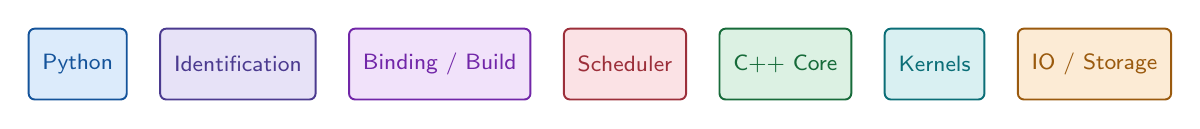
\begin{tikzpicture}[node distance=4mm]
  \node[py]    (a) {Python};
  \node[idl,   right=of a] (b) {Identification};
  \node[bind,  right=of b] (c) {Binding / Build};
  \node[sched, right=of c] (d) {Scheduler};
  \node[cpp,   right=of d] (e) {C++ Core};
  \node[kern,  right=of e] (f) {Kernels};
  \node[io,    right=of f] (g) {IO / Storage};
\end{tikzpicture}
\end{adjustbox}

\vfill
{\sffamily\small Two models, one solver engine.\\
Lindblad master equation per $k$-point, RK4, MPI $\times$ OpenMP.\par}
\vspace{4mm}
{\sffamily\footnotesize\color{Slate} Generated \today\par}
\end{titlepage}

\tableofcontents
\newpage

% ============================================================================
\section{How to read this document}
% ============================================================================

This is a structural map of the repository, not a physics paper. It answers four
questions, in this order:

\begin{enumerate}
  \item \textbf{What are the layers, and which way do they depend?} --- Section~\ref{sec:map}.
  \item \textbf{Which file needs which other file?} --- Section~\ref{sec:dep}.
  \item \textbf{What actually runs, in what order, from typing a command to the
        innermost floating-point loop?} --- Section~\ref{sec:call}.
  \item \textbf{Where does an array physically live, and what happens when it
        crosses a boundary?} --- Section~\ref{sec:mem}.
\end{enumerate}

Colour is used consistently throughout. A box's fill tells you its layer:

\medskip
\begin{center}
\begin{adjustbox}{max width=\linewidth}
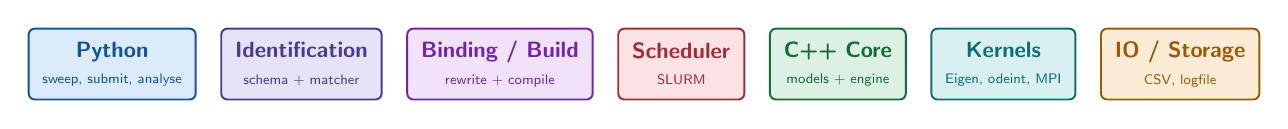
\begin{tikzpicture}[node distance=3mm]
  \node[py]    (a) {\textbf{Python}\\\tiny sweep, submit, analyse};
  \node[idl,   right=of a] (b) {\textbf{Identification}\\\tiny schema + matcher};
  \node[bind,  right=of b] (c) {\textbf{Binding / Build}\\\tiny rewrite + compile};
  \node[sched, right=of c] (d) {\textbf{Scheduler}\\\tiny SLURM};
  \node[cpp,   right=of d] (e) {\textbf{C++ Core}\\\tiny models + engine};
  \node[kern,  right=of e] (f) {\textbf{Kernels}\\\tiny Eigen, odeint, MPI};
  \node[io,    right=of f] (g) {\textbf{IO / Storage}\\\tiny CSV, logfile};
\end{tikzpicture}
\end{adjustbox}
\end{center}
\medskip

\begin{keybox}[title={A note on the word \emph{binding}}]
This project has \textbf{no in-process Python/C++ binding}. There is no
\code{.so}, no \code{.dylib}, no \code{pybind11}, \code{ctypes}, \code{Cython},
\code{cffi} or \code{f2py} anywhere in the tree, and no compiler flag ever
requests \code{-shared} or \code{-fPIC}. Python and C++ \emph{never share an
address space} and never exchange a pointer.

What sits between them instead is a \textbf{build-time and filesystem binding}:
Python rewrites the C++ source text, invokes a compiler on it, and hands the
resulting MPI executable to SLURM; the executable writes plain files; Python
reads those files back. That is the layer coloured purple throughout this
document, and it is what Section~\ref{sec:mem} describes as the memory
boundary --- a \emph{process and filesystem} boundary, marshalled by decimal
text, not a shared-buffer boundary.

This distinction is load-bearing rather than pedantic. It is why numerical
identity between the two sides is a \emph{decimal formatting contract}
(Section~\ref{sec:precision}) rather than a question of dtype and stride, and
it is why every parameter is a compile-time \code{constexpr}
(Section~\ref{sec:rewrite}).
\end{keybox}

% ============================================================================
\section{System overview}
% ============================================================================

\subsection{The four domains}

The tree is split into four directories whose dependency direction is one-way.

\begin{center}
\small
\begin{tabular}{@{}L{0.14\textwidth} L{0.44\textwidth} L{0.34\textwidth}@{}}
\toprule
\textbf{Domain} & \textbf{Responsibility} & \textbf{May import from} \\
\midrule
\code{physics/}  & C++ solver: models, engine, build. Nothing else lives here. & nothing (self-contained C++) \\
\code{workflow/} & HPC host profiles, source rewriting, compilation, job submission. & \code{analysis/} \\
\code{analysis/} & Data management, run identification, post-processing, plotting. & nothing above it \\
\code{legacy/}   & Frozen history. Never built, never imported. & --- \\
\bottomrule
\end{tabular}
\end{center}

\medskip
The single arrow \code{workflow}\,$\rightarrow$\,\code{analysis} is not a style
preference. \fn{Submitter.already\uu exists()} in \code{workflow/} must use the
\emph{same} matcher that the notebooks use to locate data. If the two ever
diverge, ``already computed'' and ``findable'' drift apart: the sweep would
either recompute points the archive already holds, or skip points nothing can
retrieve.

\subsection{The two pipelines}

Everything in the repository belongs to one of two directed pipelines that meet
at the archive.

\begin{center}
\begin{adjustbox}{max width=\textwidth}
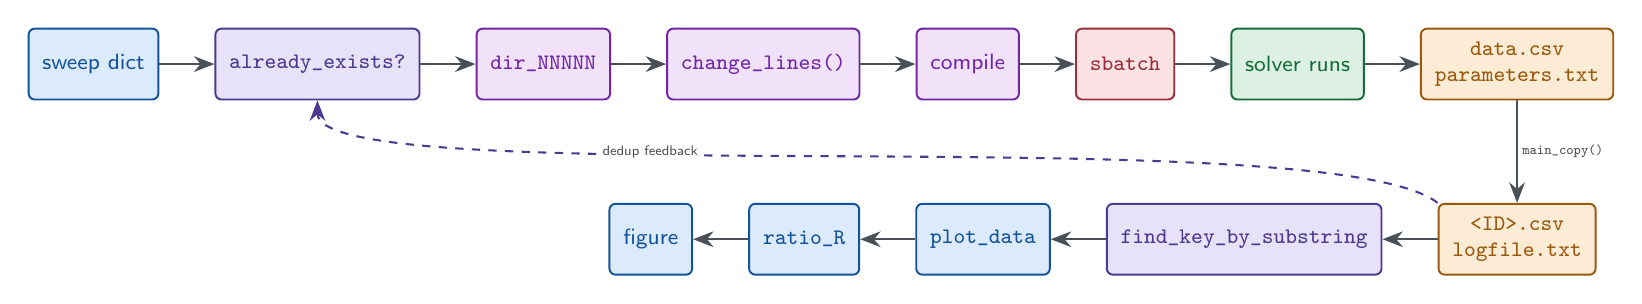
\begin{tikzpicture}[node distance=5mm and 7mm]
  \node[py]   (s1) {sweep dict};
  \node[idl,  right=of s1] (s2) {\fn{already\uu exists?}};
  \node[bind, right=of s2] (s3) {\code{dir\uu NNNNN}};
  \node[bind, right=of s3] (s4) {\fn{change\uu lines()}};
  \node[bind, right=of s4] (s5) {compile};
  \node[sched,right=of s5] (s6) {\code{sbatch}};
  \node[cpp,  right=of s6] (s7) {solver runs};
  \node[io,   right=of s7] (s8) {\code{data.csv}\\\code{parameters.txt}};

  \foreach \a/\b in {s1/s2,s2/s3,s3/s4,s4/s5,s5/s6,s6/s7,s7/s8}
     \draw[flow] (\a) -- (\b);

  \node[io,  below=13mm of s8] (a1) {\code{<ID>.csv}\\\code{logfile.txt}};
  \node[idl, left=of a1] (a2) {\fn{find\uu key\uu by\uu substring}};
  \node[py,  left=of a2] (a3) {\fn{plot\uu data}};
  \node[py,  left=of a3] (a4) {\fn{ratio\uu R}};
  \node[py,  left=of a4] (a5) {figure};

  \draw[flow] (s8) -- node[elab,right]{\fn{main\uu copy()}} (a1);
  \foreach \a/\b in {a1/a2,a2/a3,a3/a4,a4/a5}
     \draw[flow] (\a) -- (\b);

  \draw[back] (a1.north west) .. controls +(-1.4,1.1) and +(0,-1.2) ..
       node[elab,pos=0.62]{dedup feedback} (s2.south);
\end{tikzpicture}
\end{adjustbox}
\end{center}

\noindent
The dashed indigo arrow is the loop that makes the whole design cohere: the
archive feeds back into the submission decision through the very same matcher
that the analysis path uses to read it.

% ============================================================================
\section{High-level architecture map}\label{sec:map}
% ============================================================================

Figure~\ref{fig:map} is the master diagram. Read it top to bottom for the
submission path, and bottom to top for the analysis path.

\begin{figure}[p]
\centering
\begin{adjustbox}{max width=\linewidth, max totalheight=0.88\textheight, center}
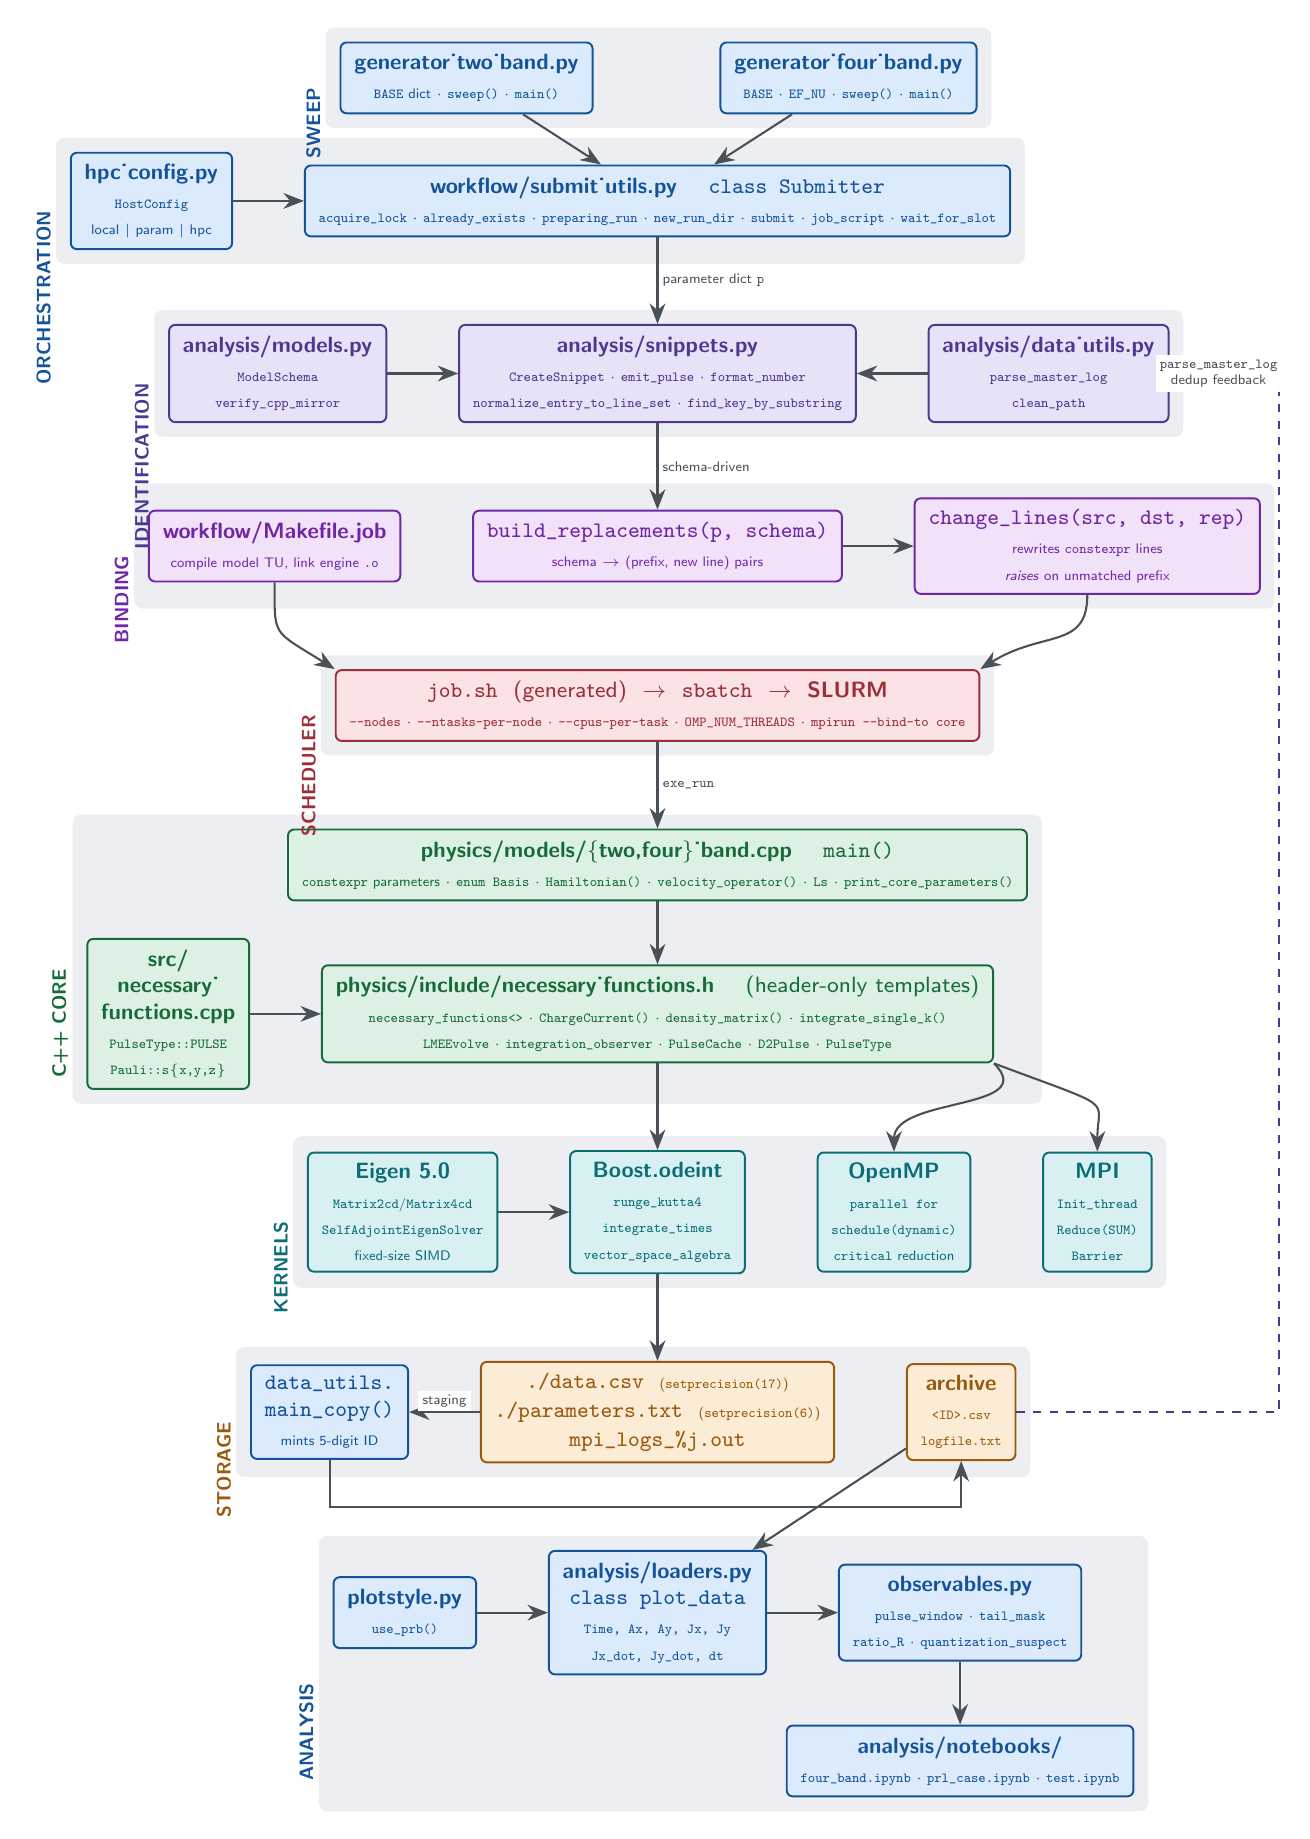
\begin{tikzpicture}[node distance=8mm and 9mm]

% ---------------------------------------------------------------- layer 1 --
\node[py] (g2) {\textbf{generator\uu two\uu band.py}\\[1pt]
                \tiny \fn{BASE} dict $\cdot$ \fn{sweep()} $\cdot$ \fn{main()}};
\node[py, right=16mm of g2] (g4) {\textbf{generator\uu four\uu band.py}\\[1pt]
                \tiny \fn{BASE} $\cdot$ \fn{EF\uu NU} $\cdot$ \fn{sweep()} $\cdot$ \fn{main()}};
\coordinate (L1c) at ($(g2)!0.5!(g4)$);

% ---------------------------------------------------------------- layer 2 --
\node[py, below=11mm of L1c] (submit)
     {\textbf{workflow/submit\uu utils.py} \quad \fn{class Submitter}\\[1pt]
      \tiny \fn{acquire\uu lock} $\cdot$ \fn{already\uu exists} $\cdot$ \fn{preparing\uu run} $\cdot$
      \fn{new\uu run\uu dir} $\cdot$ \fn{submit} $\cdot$ \fn{job\uu script} $\cdot$ \fn{wait\uu for\uu slot}};
\node[py, left=9mm of submit] (hpc)
     {\textbf{hpc\uu config.py}\\[1pt]\tiny \fn{HostConfig}\\\tiny local $\vert$ param $\vert$ hpc};

% ---------------------------------------------------------------- layer 3 --
\node[idl, below=11mm of submit] (snip)
     {\textbf{analysis/snippets.py}\\[1pt]
      \tiny \fn{CreateSnippet} $\cdot$ \fn{emit\uu pulse} $\cdot$ \fn{format\uu number}\\
      \tiny \fn{normalize\uu entry\uu to\uu line\uu set} $\cdot$ \fn{find\uu key\uu by\uu substring}};
\node[idl, left=9mm of snip] (mod)
     {\textbf{analysis/models.py}\\[1pt]\tiny \fn{ModelSchema}\\\tiny \fn{verify\uu cpp\uu mirror}};
\node[idl, right=9mm of snip] (du)
     {\textbf{analysis/data\uu utils.py}\\[1pt]\tiny \fn{parse\uu master\uu log}\\\tiny \fn{clean\uu path}};

% ---------------------------------------------------------------- layer 4 --
\node[bind, below=11mm of snip] (brep) {\fn{build\uu replacements(p, schema)}\\[1pt]
      \tiny schema $\rightarrow$ (prefix, new line) pairs};
\node[bind, right=9mm of brep] (chl) {\fn{change\uu lines(src, dst, rep)}\\[1pt]
      \tiny rewrites \fn{constexpr} lines\\\tiny \emph{raises} on unmatched prefix};
\node[bind, left=9mm of brep] (mkj) {\textbf{workflow/Makefile.job}\\[1pt]
      \tiny compile model TU, link engine \fn{.o}};

% ---------------------------------------------------------------- layer 5 --
\node[sched, below=11mm of brep] (job) {\code{job.sh}\ \ (generated)\ \ $\rightarrow$\ \ \code{sbatch}\ \ $\rightarrow$\ \ \textbf{SLURM}\\[1pt]
      \tiny \fn{--nodes} $\cdot$ \fn{--ntasks-per-node} $\cdot$ \fn{--cpus-per-task} $\cdot$ \fn{OMP\uu NUM\uu THREADS} $\cdot$ \fn{mpirun --bind-to core}};

% ---------------------------------------------------------------- layer 6 --
\node[cpp, below=11mm of job] (mainf)
     {\textbf{physics/models/\{two,four\}\uu band.cpp} \quad \fn{main()}\\[1pt]
      \tiny \fn{constexpr} parameters $\cdot$ \fn{enum Basis} $\cdot$ \fn{Hamiltonian()} $\cdot$ \fn{velocity\uu operator()}
      $\cdot$ \fn{Ls} $\cdot$ \fn{print\uu core\uu parameters()}};
\node[cpp, below=8mm of mainf] (engine)
     {\textbf{physics/include/necessary\uu functions.h} \quad (header-only templates)\\[1pt]
      \tiny \fn{necessary\uu functions<>} $\cdot$ \fn{ChargeCurrent()} $\cdot$ \fn{density\uu matrix()} $\cdot$
      \fn{integrate\uu single\uu k()}\\
      \tiny \fn{LMEEvolve} $\cdot$ \fn{integration\uu observer} $\cdot$ \fn{PulseCache} $\cdot$ \fn{D2Pulse} $\cdot$ \fn{PulseType}};
\node[cpp, left=9mm of engine] (nfcpp)
     {\textbf{src/}\\\textbf{necessary\uu}\\\textbf{functions.cpp}\\[1pt]
      \tiny \fn{PulseType::PULSE}\\\tiny \fn{Pauli::s\{x,y,z\}}};

% ---------------------------------------------------------------- layer 7 --
\node[kern, below=11mm of engine] (odeint) {\textbf{Boost.odeint}\\[1pt]
      \tiny \fn{runge\uu kutta4}\\\tiny \fn{integrate\uu times}\\\tiny \fn{vector\uu space\uu algebra}};
\node[kern, left=9mm of odeint] (eigen) {\textbf{Eigen 5.0}\\[1pt]
      \tiny \fn{Matrix2cd}/\fn{Matrix4cd}\\\tiny \fn{SelfAdjointEigenSolver}\\\tiny fixed-size SIMD};
\node[kern, right=9mm of odeint] (omp) {\textbf{OpenMP}\\[1pt]
      \tiny \fn{parallel for}\\\tiny \fn{schedule(dynamic)}\\\tiny \fn{critical} reduction};
\node[kern, right=9mm of omp] (mpi) {\textbf{MPI}\\[1pt]
      \tiny \fn{Init\uu thread}\\\tiny \fn{Reduce(SUM)}\\\tiny \fn{Barrier}};

% ---------------------------------------------------------------- layer 8 --
\node[io, below=11mm of odeint] (out) {\code{./data.csv}\ \ \tiny(\fn{setprecision(17)})\\[1pt]
      \code{./parameters.txt}\ \ \tiny(\fn{setprecision(6)})\\[1pt]
      \code{mpi\uu logs\uu \%j.out}};
\node[io, right=9mm of out] (arch) {\textbf{archive}\\[1pt]
      \tiny \code{<ID>.csv}\\\tiny \code{logfile.txt}};
\node[py, left=9mm of out] (copy) {\fn{data\uu utils.}\\\fn{main\uu copy()}\\[1pt]\tiny mints 5-digit ID};

% ---------------------------------------------------------------- layer 9 --
\node[py, below=11mm of out] (load) {\textbf{analysis/loaders.py}\\\fn{class plot\uu data}\\[1pt]
      \tiny \fn{Time, Ax, Ay, Jx, Jy}\\\tiny \fn{Jx\uu dot, Jy\uu dot, dt}};
\node[py, right=9mm of load] (obs) {\textbf{observables.py}\\[1pt]
      \tiny \fn{pulse\uu window} $\cdot$ \fn{tail\uu mask}\\\tiny \fn{ratio\uu R} $\cdot$ \fn{quantization\uu suspect}};
\node[py, left=9mm of load] (sty) {\textbf{plotstyle.py}\\[1pt]\tiny \fn{use\uu prb()}};
\node[py, below=8mm of obs] (nb) {\textbf{analysis/notebooks/}\\[1pt]
      \tiny \code{four\uu band.ipynb} $\cdot$ \code{prl\uu case.ipynb} $\cdot$ \code{test.ipynb}};

% ------------------------------------------------------------------ flows --
\draw[flow] (g2) -- (submit);
\draw[flow] (g4) -- (submit);
\draw[flow] (hpc) -- (submit);
\draw[flow] (submit) -- node[elab,right]{parameter dict \fn{p}} (snip);
\draw[flow] (mod) -- (snip);
\draw[flow] (du)  -- (snip);
\draw[flow] (snip) -- node[elab,right]{schema-driven} (brep);
\draw[flow] (brep) -- (chl);
\draw[flow] (chl.south) .. controls +(0,-0.7) and +(0.8,0.5) .. (job.north east);
\draw[flow] (mkj.south) .. controls +(0,-0.7) and +(-0.8,0.5) .. (job.north west);
\draw[flow] (job) -- node[elab,right]{\fn{exe\uu run}} (mainf);
\draw[flow] (mainf) -- (engine);
\draw[flow] (nfcpp) -- (engine);
\draw[flow] (engine) -- (odeint);
\draw[flow] (eigen) -- (odeint);
\draw[flow] (engine.south east) .. controls +(0.6,-0.6) and +(0,0.7) .. (omp.north);
\draw[flow] (engine.south east) .. controls +(1.6,-0.6) and +(0,0.7) .. (mpi.north);
\draw[flow] (odeint) -- (out);
\draw[flow] (out) -- node[elab,above]{staging} (copy);
% routed underneath the output box rather than across it
\draw[flow] (copy.south) -- ++(0,-0.6) -| (arch.south);
\draw[flow] (arch) -- (load);
\draw[flow] (load) -- (obs);
\draw[flow] (sty)  -- (load);
\draw[flow] (obs)  -- (nb);

% ---------------------------------------------------- dedup feedback loop --
% Routed along a rail to the right of every box, so it crosses nothing.
\node[coordinate, right=16mm of mpi] (rail) {};
\draw[back] (arch.east) -- (arch.east -| rail) -- (du.east -| rail) --
      node[elab,pos=0.55,align=center]{\fn{parse\uu master\uu log}\\dedup feedback} (du.east);

% ------------------------------------------------------------ layer bands --
\begin{scope}[on background layer]
  \node[band, fit=(g2)(g4), inner sep=5pt] (b1) {};
  \node[band, fit=(hpc)(submit), inner sep=5pt] (b2) {};
  \node[band, fit=(mod)(snip)(du), inner sep=5pt] (b3) {};
  \node[band, fit=(mkj)(brep)(chl), inner sep=5pt] (b4) {};
  \node[band, fit=(job), inner sep=5pt] (b5) {};
  \node[band, fit=(nfcpp)(mainf)(engine), inner sep=5pt] (b6) {};
  \node[band, fit=(eigen)(odeint)(omp)(mpi), inner sep=5pt] (b7) {};
  \node[band, fit=(copy)(out)(arch), inner sep=5pt] (b8) {};
  \node[band, fit=(sty)(load)(obs)(nb), inner sep=5pt] (b9) {};
\end{scope}

\node[bandlab, left=1.5mm of b1.west, text=PyInk]    {SWEEP};
\node[bandlab, left=1.5mm of b2.west, text=PyInk]    {ORCHESTRATION};
\node[bandlab, left=1.5mm of b3.west, text=IdInk]    {IDENTIFICATION};
\node[bandlab, left=1.5mm of b4.west, text=BindInk]  {BINDING};
\node[bandlab, left=1.5mm of b5.west, text=SchedInk] {SCHEDULER};
\node[bandlab, left=1.5mm of b6.west, text=CppInk]   {C++ CORE};
\node[bandlab, left=1.5mm of b7.west, text=KernInk]  {KERNELS};
\node[bandlab, left=1.5mm of b8.west, text=IOInk]    {STORAGE};
\node[bandlab, left=1.5mm of b9.west, text=PyInk]    {ANALYSIS};

\end{tikzpicture}
\end{adjustbox}
\caption{High-level architecture map. Solid grey arrows are the forward
submission/analysis flow; the dashed indigo arrow is the deduplication feedback
loop, which forces the submission side to reuse the analysis side's matcher.
Note that the transition from the binding layer to the C++ core is a
\emph{compiler invocation}, and the transition from the C++ core to storage is a
\emph{file write} --- there is no shared-memory interface anywhere on this
diagram.}
\label{fig:map}
\end{figure}

\clearpage

% ============================================================================
\section{End-to-end dependency graph}\label{sec:dep}
% ============================================================================

\subsection{Python module import graph}

\begin{figure}[H]
\centering
\begin{adjustbox}{width=\linewidth, max totalheight=0.80\textheight, center}
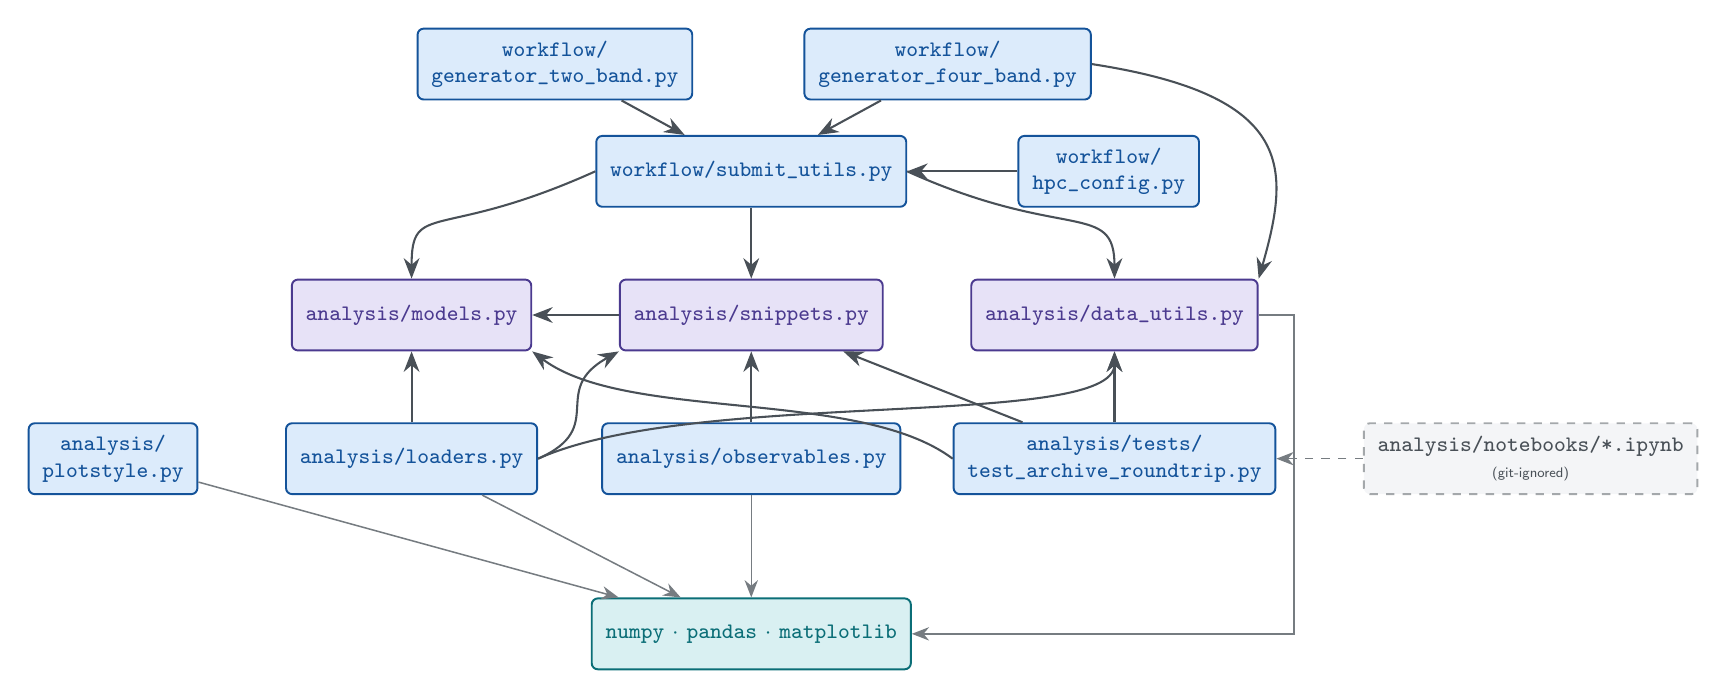
\begin{tikzpicture}[node distance=9mm and 11mm]
  \node[py] (gen4) {\code{workflow/}\\\code{generator\uu four\uu band.py}};
  \node[py, left=14mm of gen4] (gen2) {\code{workflow/}\\\code{generator\uu two\uu band.py}};
  \node[py, below=of $(gen2)!0.5!(gen4)$] (su) {\code{workflow/submit\uu utils.py}};
  \node[py, right=14mm of su] (hc) {\code{workflow/}\\\code{hpc\uu config.py}};

  \node[idl, below=of su] (sn) {\code{analysis/snippets.py}};
  \node[idl, left=11mm of sn] (md) {\code{analysis/models.py}};
  \node[idl, right=11mm of sn] (dt) {\code{analysis/data\uu utils.py}};

  \node[py, below=of md] (ld) {\code{analysis/loaders.py}};
  \node[py, below=of sn] (ob) {\code{analysis/observables.py}};
  \node[py, below=of dt] (ts) {\code{analysis/tests/}\\\code{test\uu archive\uu roundtrip.py}};
  \node[py, left=11mm of ld] (ps) {\code{analysis/}\\\code{plotstyle.py}};

  \node[kern, below=13mm of ob] (np) {\code{numpy} $\cdot$ \code{pandas} $\cdot$ \code{matplotlib}};
  \node[ghost, right=11mm of ts] (nbk) {\code{analysis/notebooks/*.ipynb}\\\tiny (git-ignored)};

  \draw[flow] (gen2) -- (su);
  \draw[flow] (gen4) -- (su);
  \draw[flow] (hc)   -- (su);
  \draw[flow] (su)   -- (sn);
  \draw[flow] (su.west) .. controls +(-2.0,-0.9) and +(0,1.0) .. (md.north);
  \draw[flow] (su.east) .. controls +(2.0,-0.9) and +(0,1.0) .. (dt.north);
  \draw[flow] (gen4.east) .. controls +(2.6,-0.4) and +(0.4,1.4) .. (dt.north east);
  \draw[flow] (sn) -- (md);
  \draw[flow] (ld) -- (md);
  \draw[flow] (ld.east) .. controls +(0.9,0.4) and +(-0.9,-0.5) .. (sn.south west);
  \draw[flow] (ld.east) .. controls +(2.0,0.9) and +(0,-1.0) .. (dt.south);
  \draw[flow] (ob) -- (sn);
  \draw[flow] (ts) -- (sn);
  \draw[flow] (ts) -- (dt);
  \draw[flow] (ts.west) .. controls +(-1.2,0.9) and +(1.2,-0.9) .. (md.south east);
  \draw[thin] (ld) -- (np);
  \draw[thin] (ob) -- (np);
  \draw[thin] (ps) -- (np);
  % routed around the right rather than straight down through the tests box
  \draw[thin] (dt.east) -- ++(0.45,0) |- (np.east);
  \draw[thin, dashed] (nbk) -- (ts);
\end{tikzpicture}
\end{adjustbox}
\caption{Python import graph. Every arrow points from importer to imported.
Note that no arrow leaves \code{analysis/} and enters \code{workflow/}: the
dependency is strictly one-way. \code{workflow/} bootstraps this by inserting
\code{analysis/} onto \code{sys.path} at import time.}
\end{figure}

\subsection{Python module inventory}

\begin{center}
\scriptsize
\begin{longtable}{@{}L{0.20\textwidth} L{0.40\textwidth} L{0.34\textwidth}@{}}
\toprule
\textbf{File} & \textbf{Defines} & \textbf{Imports} \\
\midrule
\endfirsthead
\toprule
\textbf{File} & \textbf{Defines} & \textbf{Imports} \\
\midrule
\endhead
\code{workflow/}\newline\code{generator\uu two\uu band.py}
 & \fn{BASE} dict, \fn{sweep()}, \fn{main()}, \fn{ARCHIVE}
 & \fn{argparse}, \fn{numpy}, \fn{data\uu utils.clean\uu path}, \fn{models.TWO\uu BAND}, \fn{submit\uu utils.Submitter} \\
\addlinespace
\code{workflow/}\newline\code{generator\uu four\uu band.py}
 & \fn{BASE} dict, \fn{EF\uu NU} table, \fn{sweep()}, \fn{main()}
 & as above, with \fn{models.FOUR\uu BAND} \\
\addlinespace
\code{workflow/}\newline\code{submit\uu utils.py}
 & \fn{class Submitter} (\fn{acquire\uu lock}, \fn{release\uu lock},
   \fn{already\uu exists}, \fn{is\uu job\uu complete}, \fn{preparing\uu run},
   \fn{new\uu run\uu dir}, \fn{job\uu script}, \fn{record\uu directory},
   \fn{submit}, \fn{\uu quarantine}, \fn{wait\uu for\uu slot});
   \fn{count\uu running\uu jobs}, \fn{get\uu active\uu job\uu info},
   \fn{\uu parse\uu cached}, \fn{change\uu lines}, \fn{build\uu replacements},
   \fn{\uu CPP\uu ENUM}
 & \fn{atexit}, \fn{os}, \fn{random}, \fn{shutil}, \fn{subprocess}, \fn{sys},
   \fn{time}, \fn{functools.lru\uu cache}, \fn{pathlib};\newline
   \fn{data\uu utils}, \fn{models}, \fn{snippets}, \fn{hpc\uu config} \\
\addlinespace
\code{workflow/}\newline\code{hpc\uu config.py}
 & \fn{detect\uu host()}, \fn{class HostConfig}, \fn{PARAM}, \fn{HPC}, \fn{LOCAL}, \fn{HOSTS}, \fn{get()}
 & \fn{os}, \fn{dataclasses}, \fn{pathlib} \\
\midrule
\code{analysis/}\newline\code{models.py}
 & \fn{class ModelSchema}, \fn{TWO\uu BAND}, \fn{FOUR\uu BAND}, \fn{MODELS},
   \fn{by\uu system()}, \fn{cpp\uu emitted\uu keys()}, \fn{verify\uu cpp\uu mirror()}
 & \fn{dataclasses}, \fn{pathlib}, \fn{re} \\
\addlinespace
\code{analysis/}\newline\code{snippets.py}
 & \fn{format\uu number}, \fn{float\uu number}, \fn{get\uu param},
   \fn{get\uu vector\uu param}, \fn{resolve},
   \fn{normalize\uu entry\uu to\uu line\uu set}, \fn{emit\uu pulse},
   \fn{DEFAULT\uu IGNORE\uu PATTERNS}, \fn{class CreateSnippet},
   \fn{find\uu key\uu by\uu substring}, \fn{show\uu nearest\uu candidates}
 & \fn{numpy}, \fn{textwrap.dedent}, \fn{models} \\
\addlinespace
\code{analysis/}\newline\code{data\uu utils.py}
 & \fn{clean\uu path}, \fn{parse\uu complex}, \fn{parse\uu master\uu log},
   \fn{merge\uu and\uu sort\uu csv}, \fn{merge\uu and\uu minimize\uu csv},
   \fn{delete\uu contents\uu from\uu log}, \fn{main\uu delete},
   \fn{main\uu copy}, \fn{sync\uu simulation\uu data}
 & \fn{re}, \fn{os}, \fn{platform}, \fn{pathlib}, \fn{pandas}, \fn{numpy},
   \fn{shutil}, \fn{random} \\
\addlinespace
\code{analysis/}\newline\code{loaders.py}
 & \fn{class plot\uu data}, \fn{\uu system\uu of()}
 & \fn{pathlib}, \fn{numpy}, \fn{pandas}, \fn{data\uu utils}, \fn{models}, \fn{snippets} \\
\addlinespace
\code{analysis/}\newline\code{observables.py}
 & \fn{pulse\uu window()}, \fn{tail\uu mask()}, \fn{ratio\uu R()}, \fn{quantization\uu suspect()}
 & \fn{numpy}, \fn{snippets.get\uu param} \\
\addlinespace
\code{analysis/}\newline\code{plotstyle.py}
 & \fn{use\uu prb()} (APS PRB \fn{rcParams})
 & \fn{matplotlib} \\
\addlinespace
\code{analysis/tests/}\newline\code{test\uu archive\uu roundtrip.py}
 & \fn{params\uu from\uu entry()}, round-trip acceptance test over the real archive
 & \fn{sys}, \fn{pathlib}, \fn{data\uu utils}, \fn{models}, \fn{snippets} \\
\bottomrule
\end{longtable}
\end{center}

\subsection{C++ translation units, headers and artifacts}

There are exactly \textbf{three} C++ source files and \textbf{one} project
header. Every executable is built from two object files.

\begin{center}
\scriptsize
\begin{tabular}{@{}L{0.24\textwidth} L{0.42\textwidth} L{0.28\textwidth}@{}}
\toprule
\textbf{File} & \textbf{Defines} & \textbf{Includes} \\
\midrule
\code{physics/include/}\newline\code{necessary\uu functions.h}
 & \fn{max\uu threads}, \fn{thread\uu id}, \fn{c\uu d}, namespace \fn{Pauli}
   (decls), namespace \fn{constants} (\fn{z}, \fn{PI}, \fn{e}),
   \fn{class ProgramTimer}, \fn{printCurrentDateTime},
   \fn{complex\uu to\uu string}, \fn{Commutator}, \fn{AntiCommutator},
   \fn{enum class PulseKind}, \fn{operator<<}, \fn{class PulseType},
   \fn{class D2Pulse}, \fn{class PulseCache},
   \fn{template class LMEEvolve}, \fn{template class integration\uu observer},
   \fn{template integrate\uu single\uu k}, \fn{template class necessary\uu functions}
 & \fn{omp.h}, \fn{Eigen/\brk Dense},\newline
   \fn{unsupported/\brk Eigen/\brk MatrixFunctions},\newline
   \fn{boost/\brk numeric/\brk odeint.hpp},\newline
   \fn{boost/\brk .../\brk external/\brk eigen/\brk eigen.hpp},\newline
   \fn{mpi.h} \\
\addlinespace
\code{physics/src/}\newline\code{necessary\uu functions.cpp}
 & \fn{Pauli::\brk sx/\brk sy/\brk sz} (definitions),
   \fn{ProgramTimer::\brk \{ctor,\brk stop,\brk formatted\}},
   \fn{printCurrentDateTime}, \fn{PulseType::\brk \{ctor,\brk gaussian,\brk sin2,\brk
   gaussian\uu envelope,\brk sin\uu envelope,\brk Sin,\brk Cos,\brk PULSE\}}
 & \fn{iomanip}, \fn{necessary\uu functions.h} \\
\addlinespace
\code{physics/models/}\newline\code{two\uu band.cpp}
 & \fn{constexpr} parameters ($\alpha,\beta,\delta,m,\dots$),
   \fn{enum Basis\brk \{State0,\brk State1\}}, \fn{shifted\uu momentum},
   \fn{off\uu diag}, \fn{D\uu off\uu diag}, \fn{Hamiltonian} (\fn{Matrix2cd}),
   \fn{velocity\uu operator}, \fn{L1}, \fn{L2}, \fn{Ls},
   \fn{main()} with the \fn{print\uu core\uu parameters} lambda
 & \fn{fstream}, \fn{necessary\uu functions.h},\newline
   \fn{unsupported/\brk Eigen/\brk KroneckerProduct} \\
\addlinespace
\code{physics/models/}\newline\code{four\uu band.cpp}
 & \fn{constexpr} parameters ($V,v,v_3,\gamma_1,\dots$),
   \fn{enum Basis\brk \{State0..\brk State3\}}, \fn{shifted\uu momentum},
   \fn{term\uu v}, \fn{term\uu v3}, \fn{D\uu term\uu v}, \fn{D\uu term\uu v3},
   \fn{Hamiltonian} (\fn{Matrix4cd}), \fn{VelocityOperatorConst},
   \fn{velocity\uu operator}, \fn{L1..L4}, \fn{Ls}, \fn{main()}
 & as above \\
\bottomrule
\end{tabular}
\end{center}

\medskip

\begin{center}
\scriptsize
\begin{tabular}{@{}L{0.30\textwidth} L{0.30\textwidth} L{0.34\textwidth}@{}}
\toprule
\textbf{Artifact} & \textbf{Built from} & \textbf{Kind} \\
\midrule
\code{build/\$(HOST)/necessary\uu functions.o} & \code{src/necessary\uu functions.cpp} & static object, built \emph{once} per host \\
\code{build/\$(HOST)/two\uu band.o}   & \code{models/two\uu band.cpp}   & static object \\
\code{build/\$(HOST)/four\uu band.o}  & \code{models/four\uu band.cpp}  & static object \\
\code{build/\$(HOST)/two\uu band}     & both \code{.o} above            & MPI executable \\
\code{build/\$(HOST)/four\uu band}    & both \code{.o} above            & MPI executable \\
\code{dir\uu NNNNN/exe\uu run}        & rewritten \code{<model>.cpp} + shared engine \code{.o} & MPI executable, one per run \\
\midrule
\multicolumn{3}{@{}l@{}}{\emph{No shared library is produced anywhere.} There is no \code{.so} and no \code{.dylib} target in either Makefile.}\\
\bottomrule
\end{tabular}
\end{center}

\subsection{Why two executables and not one}

The matrix dimension is fixed at compile time. \fn{necessary\uu functions<>}
carries
\begin{center}\code{static\uu assert(M\uu compileM != Eigen::Dynamic)}\end{center}
so \fn{Eigen::Matrix2cd} and \fn{Eigen::Matrix4cd} instantiate genuinely
different template code, with different stack layouts and different SIMD
kernels. A $2\times2$ and a $4\times4$ model cannot share one binary. This is
deliberate: fixed-size Eigen types are stack-allocated and unrolled, which is
where most of the solver's speed comes from.

\subsection{Third-party dependencies}

\begin{center}
\scriptsize
\begin{tabular}{@{}L{0.20\textwidth} L{0.22\textwidth} L{0.50\textwidth}@{}}
\toprule
\textbf{Dependency} & \textbf{Used by} & \textbf{What for} \\
\midrule
Eigen 5.0.0 (header-only)   & C++ core   & fixed-size complex matrices, \fn{SelfAdjointEigenSolver} for the initial density matrix \\
Boost 1.89.0 \fn{odeint}    & C++ core   & \fn{runge\uu kutta4} stepper, \fn{integrate\uu times} driver, \fn{vector\uu space\uu algebra} adaptor for Eigen state types \\
OpenMPI 5.0.8               & C++ core   & rank-level decomposition over the $k$-grid, \fn{MPI\uu Reduce} of the current \\
OpenMP                      & C++ core   & thread-level parallelism inside a rank \\
NumPy / pandas              & analysis   & CSV load, \fn{np.diff} derivatives, array maths \\
Matplotlib                  & analysis   & figures, PRB \fn{rcParams} \\
SLURM (\fn{sbatch}, \fn{squeue}) & workflow & job submission and throttling \\
\bottomrule
\end{tabular}
\end{center}

% ============================================================================
\section{Function call graph and execution path}\label{sec:call}
% ============================================================================

The lifetime of one parameter point has four phases. Phase A runs on the login
node in Python; phase B runs on compute nodes in C++; phase C is an archival
step in Python; phase D is analysis, in Python.

\subsection{Phase A --- submission (Python, login node)}

\begin{figure}[H]
\centering
\begin{adjustbox}{width=\linewidth, max totalheight=0.80\textheight, center}
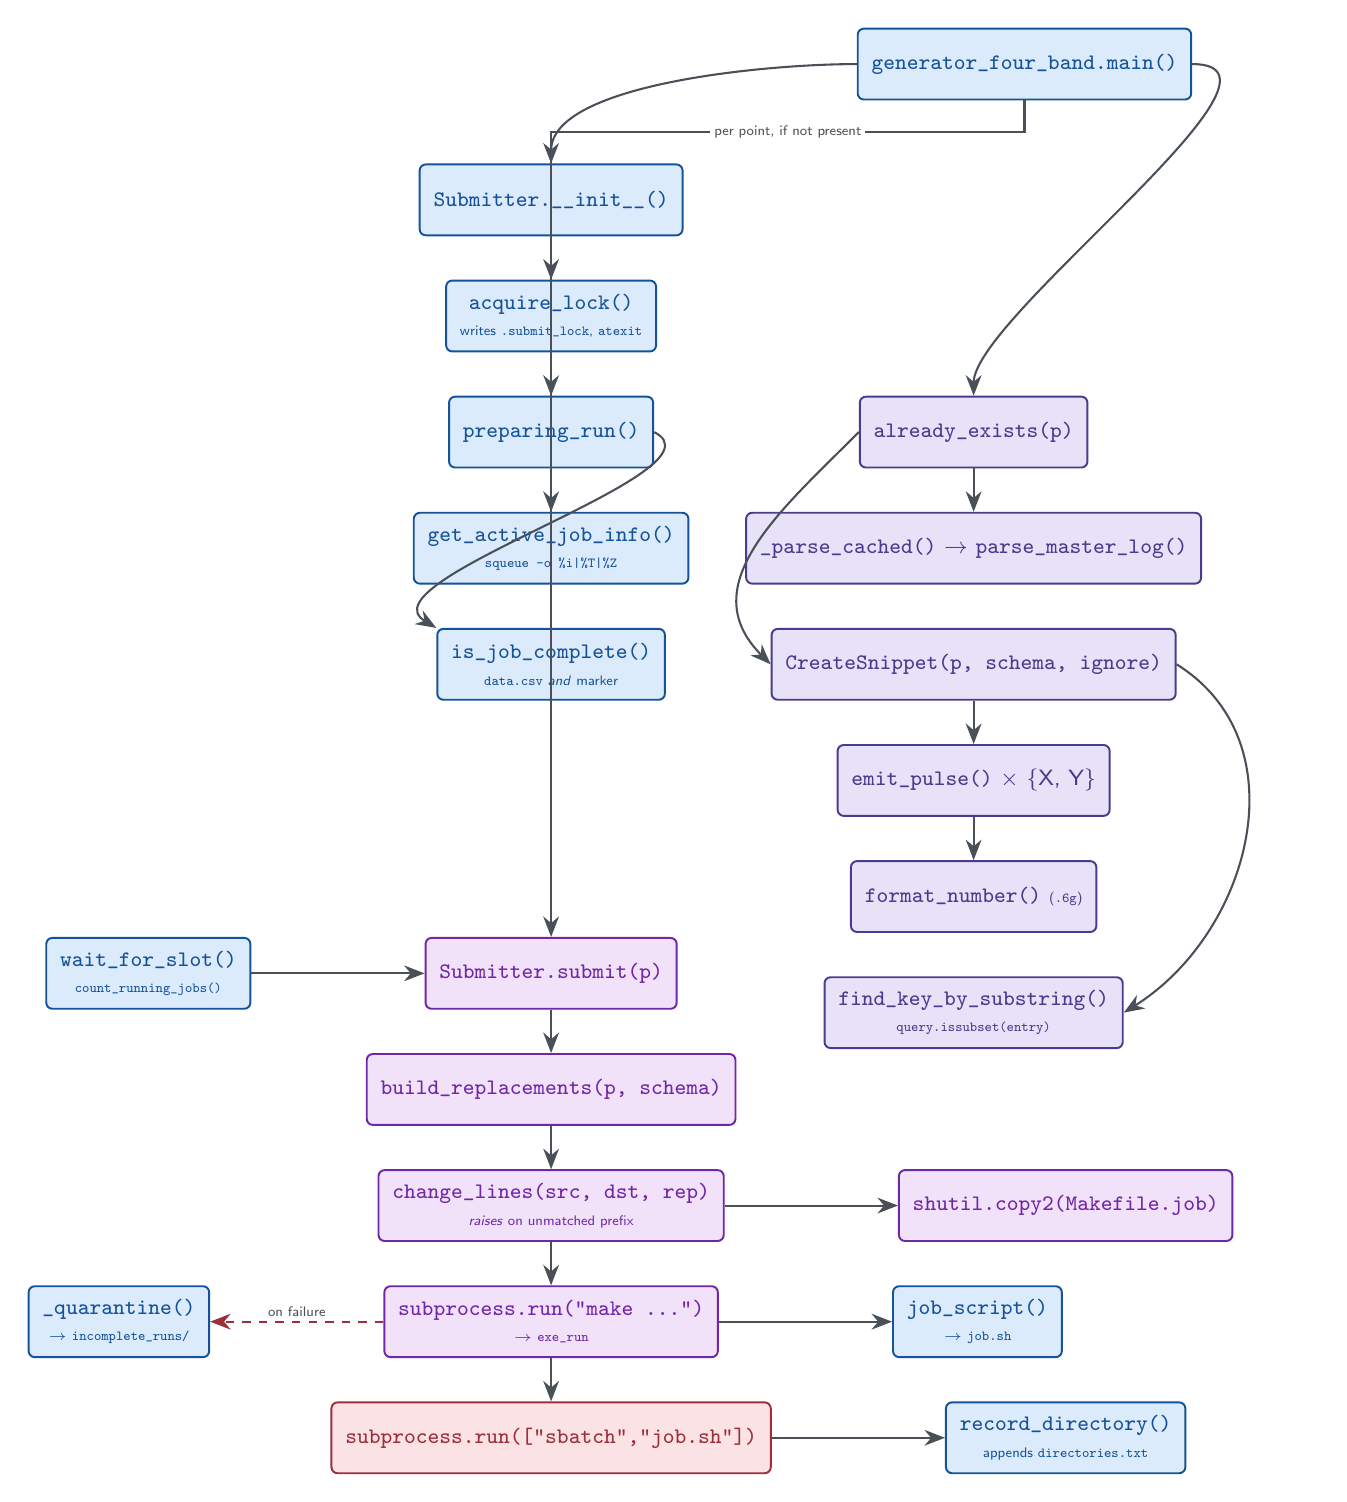
\begin{tikzpicture}[node distance=5.5mm and 12mm,
                    every node/.append style={font=\scriptsize\sffamily}]

  \node[py] (m) {\fn{generator\uu four\uu band.main()}};
  \node[py, below left=8mm and 22mm of m] (mk) {\fn{Submitter.\uu\uu init\uu\uu()}};
  \node[py, below=of mk] (lk) {\fn{acquire\uu lock()}\\\tiny writes \code{.submit\uu lock}, \fn{atexit}};
  \node[py, below=of lk] (pr) {\fn{preparing\uu run()}};
  \node[py, below=of pr] (aj) {\fn{get\uu active\uu job\uu info()}\\\tiny \code{squeue -o \%i|\%T|\%Z}};
  \node[py, below=of aj] (ic) {\fn{is\uu job\uu complete()}\\\tiny \code{data.csv} \emph{and} marker};

  \node[idl, right=26mm of pr] (ae) {\fn{already\uu exists(p)}};
  \node[idl, below=of ae] (pl) {\fn{\uu parse\uu cached()} $\rightarrow$ \fn{parse\uu master\uu log()}};
  \node[idl, below=of pl] (cs) {\fn{CreateSnippet(p, schema, ignore)}};
  \node[idl, below=of cs] (ep) {\fn{emit\uu pulse()} $\times$ \{X, Y\}};
  \node[idl, below=of ep] (fm) {\fn{format\uu number()} \tiny(\code{.6g})};
  \node[idl, below=of fm] (fk) {\fn{find\uu key\uu by\uu substring()}\\\tiny \fn{query.issubset(entry)}};

  \node[bind, below=30mm of ic] (sb) {\fn{Submitter.submit(p)}};
  \node[bind, below=of sb] (br) {\fn{build\uu replacements(p, schema)}};
  \node[bind, below=of br] (cl) {\fn{change\uu lines(src, dst, rep)}\\\tiny \emph{raises} on unmatched prefix};
  \node[bind, right=22mm of cl] (cp) {\fn{shutil.copy2(Makefile.job)}};
  \node[bind, below=of cl] (mkc) {\fn{subprocess.run("make ...")}\\\tiny $\rightarrow$ \code{exe\uu run}};
  \node[py,   right=22mm of mkc] (js) {\fn{job\uu script()}\\\tiny $\rightarrow$ \code{job.sh}};
  \node[sched,below=of mkc] (sba) {\fn{subprocess.run(["sbatch","job.sh"])}};
  \node[py,   right=22mm of sba] (rd) {\fn{record\uu directory()}\\\tiny appends \code{directories.txt}};
  \node[py,   left=22mm of mkc] (qn) {\fn{\uu quarantine()}\\\tiny $\rightarrow$ \code{incomplete\uu runs/}};
  \node[py,   left=22mm of sb]  (ws) {\fn{wait\uu for\uu slot()}\\\tiny \fn{count\uu running\uu jobs()}};

  \draw[flow] (m.west) .. controls +(-1.2,0) and +(0,1.0) .. (mk.north);
  \draw[flow] (mk) -- (lk);
  \draw[flow] (lk) -- (pr);
  \draw[flow] (pr) -- (aj);
  \draw[flow] (pr.east) .. controls +(1.0,-0.5) and +(-1.0,0.6) .. (ic.north west);
  \draw[flow] (m.east) .. controls +(1.6,0) and +(0,1.0) .. (ae.north);
  \draw[flow] (ae) -- (pl);
  \draw[flow] (ae.west) .. controls +(-1.0,-1.0) and +(-1.0,1.0) .. (cs.west);
  \draw[flow] (cs) -- (ep);
  \draw[flow] (ep) -- (fm);
  \draw[flow] (cs.east) .. controls +(1.6,-1.0) and +(1.6,1.0) .. (fk.east);
  \draw[flow] (m.south) -- ++(0,-0.4) -| node[elab,pos=0.25]{per point, if not present} (sb.north);
  \draw[flow] (sb) -- (br);
  \draw[flow] (br) -- (cl);
  \draw[flow] (cl) -- (cp);
  \draw[flow] (cl) -- (mkc);
  \draw[flow] (mkc) -- (js);
  \draw[flow] (mkc) -- (sba);
  \draw[flow] (sba) -- (rd);
  \draw[flow, draw=SchedInk, dashed] (mkc) -- node[elab,above]{on failure} (qn);
  \draw[flow] (ws) -- (sb);
\end{tikzpicture}
\end{adjustbox}
\caption{Phase A call graph. The indigo column is the identification layer,
entered from both the deduplication check and (indirectly, through
\fn{build\uu replacements}) the source-rewriting step, which is what keeps the
two in sync.}
\end{figure}

\subsubsection{The source-rewriting mechanism}\label{sec:rewrite}

Model parameters are compile-time \fn{constexpr} in \code{physics/models/*.cpp}.
A parameter point is realised by rewriting that source and recompiling. This is
the settled mechanism, not a stopgap.

\begin{center}
\scriptsize
\begin{tabular}{@{}L{0.30\textwidth} L{0.62\textwidth}@{}}
\toprule
\textbf{Step} & \textbf{Effect} \\
\midrule
\fn{build\uu replacements(p, schema)} & Walks \fn{schema.scalars} and the pulse keys, producing
   \code{("constexpr double ef =", "constexpr double ef = 0.72;")} pairs.
   Derived from \code{analysis/models.py}, so adding a parameter is one edit there rather than thirty call sites. \\
\fn{change\uu lines(src, dst, rep)} & Reads the source, replaces each whole line whose stripped form starts with the prefix, writes the copy into \code{dir\uu NNNNN/<model>.cpp}.
   \textbf{Raises} \fn{ValueError} on any unmatched prefix --- a silent miss would run a job with the wrong parameter and archive it under the wrong label. \\
\code{Makefile.job} & Copied in as \code{Makefile}; compiles only the rewritten model TU and links the pre-built engine object. \\
\bottomrule
\end{tabular}
\end{center}

\begin{sloppypar}
\noindent Three places must agree when a parameter is added: the \fn{constexpr}
in the model source, \fn{print\uu core\uu parameters()} next to it, and
\fn{ModelSchema.scalars}. \fn{verify\uu cpp\uu mirror()} reads the \code{.cpp}
and catches the third going stale --- C++ cannot import the Python schema, so
this check is the only thing standing between the project and silent emitter
drift.
\end{sloppypar}

\subsection{Phase B --- the compute kernel (C++, compute nodes)}

\begin{figure}[p]
\centering
\begin{adjustbox}{width=\linewidth, max totalheight=0.84\textheight, center}
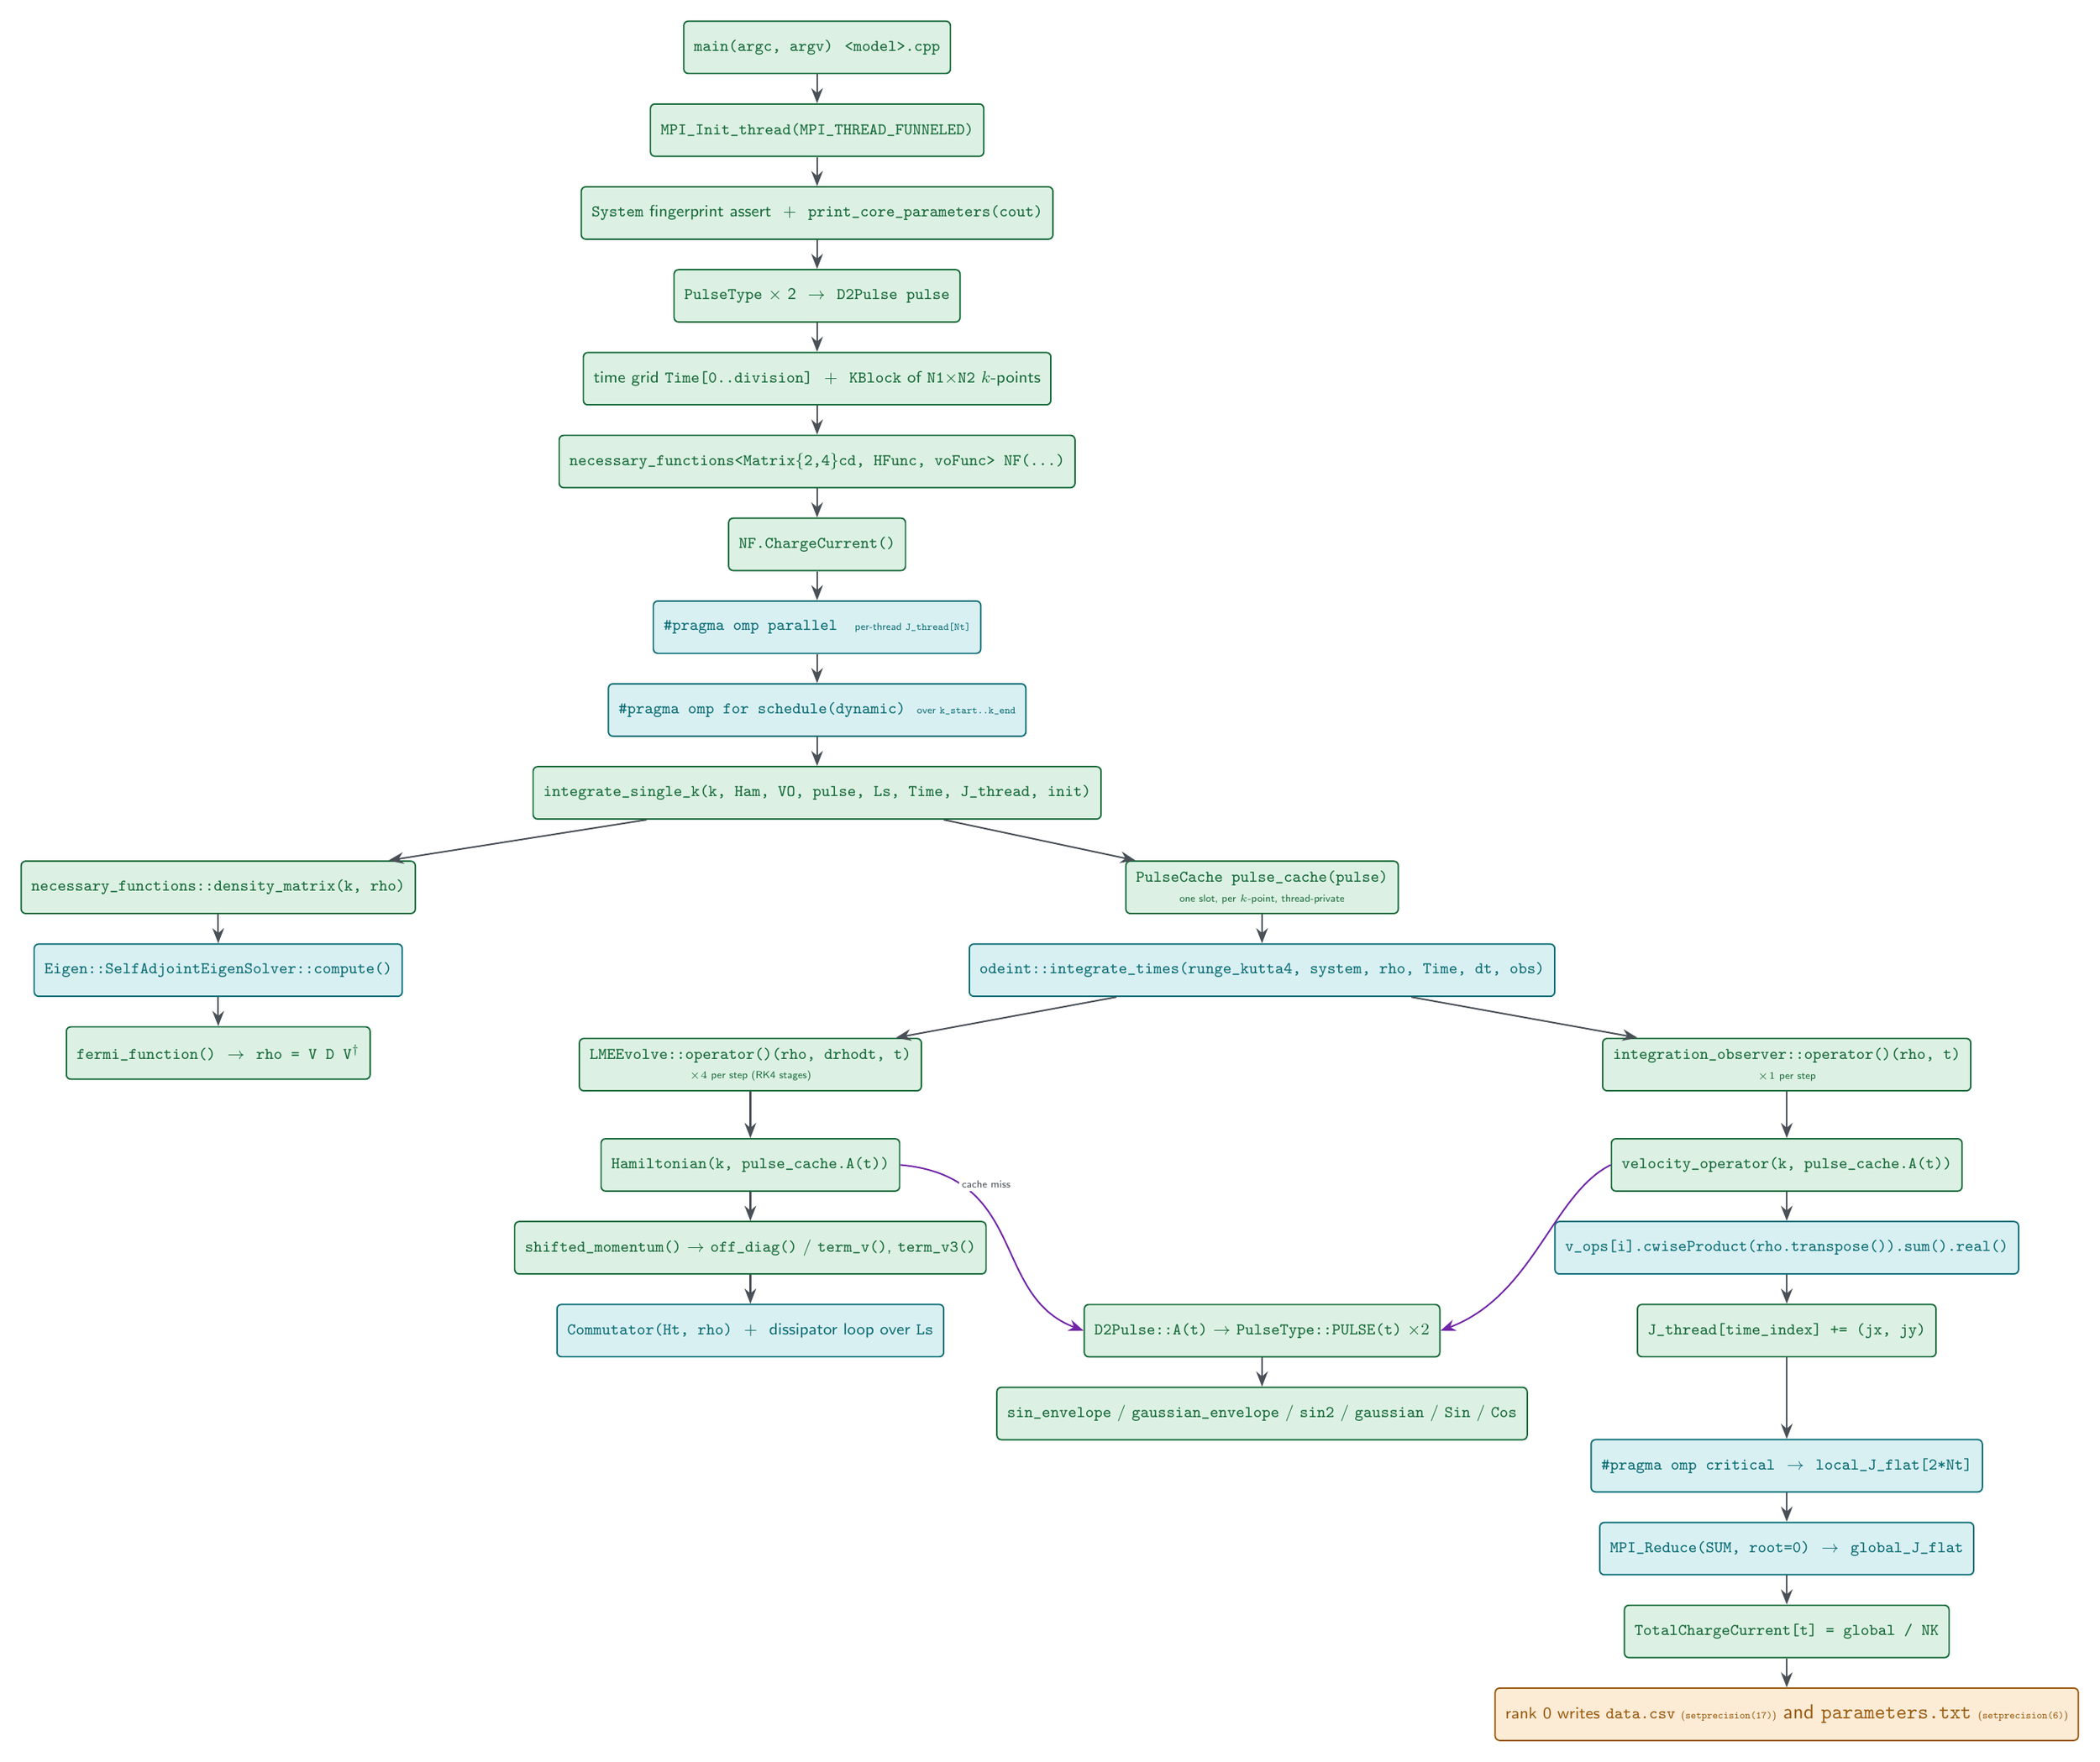
\begin{tikzpicture}[node distance=5mm and 14mm,
                    every node/.append style={font=\scriptsize\sffamily}]

  \node[cpp] (main) {\fn{main(argc, argv)}\ \ \code{<model>.cpp}};
  \node[cpp, below=of main] (mpii) {\fn{MPI\uu Init\uu thread(MPI\uu THREAD\uu FUNNELED)}};
  \node[cpp, below=of mpii] (chk) {\fn{System} fingerprint assert\ \ +\ \ \fn{print\uu core\uu parameters(cout)}};
  \node[cpp, below=of chk] (pul) {\fn{PulseType} $\times$ 2\ \ $\rightarrow$\ \ \fn{D2Pulse pulse}};
  \node[cpp, below=of pul] (grid) {time grid \fn{Time[0..division]}\ \ +\ \ \fn{KBlock} of \fn{N1}$\times$\fn{N2} $k$-points};
  \node[cpp, below=of grid] (nf) {\fn{necessary\uu functions<Matrix\{2,4\}cd, HFunc, voFunc> NF(...)}};
  \node[cpp, below=of nf] (cc) {\fn{NF.ChargeCurrent()}};

  \node[kern, below=of cc] (par) {\code{\#pragma omp parallel}\ \ \ \tiny per-thread \fn{J\uu thread[Nt]}};
  \node[kern, below=of par] (fo) {\code{\#pragma omp for schedule(dynamic)}\ \ \tiny over \fn{k\uu start..k\uu end}};
  \node[cpp,  below=of fo] (isk) {\fn{integrate\uu single\uu k(k, Ham, VO, pulse, Ls, Time, J\uu thread, init)}};

  \node[cpp, below left=7mm and 20mm of isk] (dm) {\fn{necessary\uu functions::density\uu matrix(k, rho)}};
  \node[kern, below=of dm] (es) {\fn{Eigen::SelfAdjointEigenSolver::compute()}};
  \node[cpp, below=of es] (ff) {\fn{fermi\uu function()}\ \ $\rightarrow$\ \ \fn{rho = V D V}$^\dagger$};

  \node[cpp, below right=7mm and 4mm of isk] (pc) {\fn{PulseCache pulse\uu cache(pulse)}\\\tiny one slot, per $k$-point, thread-private};
  \node[kern, below=of pc] (it) {\fn{odeint::integrate\uu times(runge\uu kutta4, system, rho, Time, dt, obs)}};

  \node[cpp, below left=7mm and 8mm of it] (lme) {\fn{LMEEvolve::operator()(rho, drhodt, t)}\\\tiny $\times 4$ per step (RK4 stages)};
  \node[cpp, below right=7mm and 8mm of it] (obsv) {\fn{integration\uu observer::operator()(rho, t)}\\\tiny $\times 1$ per step};

  \node[cpp, below=8mm of lme] (ham) {\fn{Hamiltonian(k, pulse\uu cache.A(t))}};
  \node[cpp, below=of ham] (odg) {\fn{shifted\uu momentum()} $\rightarrow$ \fn{off\uu diag()} / \fn{term\uu v()}, \fn{term\uu v3()}};
  \node[kern, below=of odg] (com) {\fn{Commutator(Ht, rho)}\ \ +\ \ dissipator loop over \fn{Ls}};

  \node[cpp, below=8mm of obsv] (vo) {\fn{velocity\uu operator(k, pulse\uu cache.A(t))}};
  \node[kern, below=of vo] (tr) {\fn{v\uu ops[i].cwiseProduct(rho.transpose()).sum().real()}};
  \node[cpp, below=of tr] (acc) {\fn{J\uu thread[time\uu index] += (jx, jy)}};

  \node[cpp, below=of pc, yshift=-62mm] (pcA) {\fn{D2Pulse::A(t)} $\rightarrow$ \fn{PulseType::PULSE(t)} $\times 2$};
  \node[cpp, below=of pcA] (shape) {\fn{sin\uu envelope} / \fn{gaussian\uu envelope} / \fn{sin2} / \fn{gaussian} / \fn{Sin} / \fn{Cos}};

  \node[kern, below=14mm of acc] (crit) {\code{\#pragma omp critical}\ \ $\rightarrow$\ \ \fn{local\uu J\uu flat[2*Nt]}};
  \node[kern, below=of crit] (red) {\fn{MPI\uu Reduce(SUM, root=0)}\ \ $\rightarrow$\ \ \fn{global\uu J\uu flat}};
  \node[cpp,  below=of red] (norm) {\fn{TotalChargeCurrent[t] = global / NK}};
  \node[io,   below=of norm] (wr) {rank 0 writes \code{data.csv} \tiny(\fn{setprecision(17)})\normalsize\ and \code{parameters.txt} \tiny(\fn{setprecision(6)})};

  \foreach \a/\b in {main/mpii,mpii/chk,chk/pul,pul/grid,grid/nf,nf/cc,cc/par,par/fo,fo/isk}
     \draw[flow] (\a) -- (\b);
  \draw[flow] (isk) -- (dm);
  \draw[flow] (dm) -- (es);
  \draw[flow] (es) -- (ff);
  \draw[flow] (isk) -- (pc);
  \draw[flow] (pc) -- (it);
  \draw[flow] (it) -- (lme);
  \draw[flow] (it) -- (obsv);
  \draw[flow] (lme) -- (ham);
  \draw[flow] (ham) -- (odg);
  \draw[flow] (odg) -- (com);
  \draw[flow] (obsv) -- (vo);
  \draw[flow] (vo) -- (tr);
  \draw[flow] (tr) -- (acc);
  \draw[flow, draw=BindInk] (ham.east) .. controls +(2.2,-0.2) and +(-1.6,0.6) ..
        node[elab,pos=0.22,above right=-1mm and -1mm]{cache miss} (pcA.west);
  \draw[flow, draw=BindInk] (vo.west)  .. controls +(-1.0,-0.5) and +(1.6,0.6) .. (pcA.east);
  \draw[flow] (pcA) -- (shape);
  \draw[flow] (acc) -- (crit);
  \draw[flow] (crit) -- (red);
  \draw[flow] (red) -- (norm);
  \draw[flow] (norm) -- (wr);
\end{tikzpicture}
\end{adjustbox}
\caption{Phase B call graph, from \fn{main()} down to the innermost numerical
kernels. Purple arrows mark the two call sites that consult the pulse cache;
both are served from one evaluation whenever they land on the same $t$.}
\label{fig:kernel}
\end{figure}


\subsubsection{Innermost-loop cost model}\label{sec:cost}

Per \emph{accepted RK4 timestep}, per $k$-point, the following calls occur.
\fn{runge\uu kutta4} is a classical four-stage stepper evaluating the system at
$t$, $t+\tfrac{dt}{2}$ (twice, sharing one time value), and $t+dt$;
\fn{integrate\uu times} calls the observer once per grid point.

\begin{center}
\scriptsize
\begin{tabular}{@{}L{0.40\textwidth} c c L{0.30\textwidth}@{}}
\toprule
\textbf{Callee} & \textbf{Before} & \textbf{After} & \textbf{Why} \\
\midrule
\fn{LMEEvolve::operator()}         & 4 & 4 & the four RK4 stages \\
\fn{integration\uu observer::operator()} & 1 & 1 & one grid point \\
\fn{Hamiltonian(k, A)}             & 4 & 4 & one per stage \\
\fn{velocity\uu operator(k, A)}    & 1 & 1 & one per observation \\
\midrule
\fn{D2Pulse::A(t)}                 & 5 & \textbf{2} & cache serves $t$ (from the previous step's final stage) and the repeated $t+\tfrac{dt}{2}$ \\
\fn{PulseType::PULSE(t)}           & 10 & \textbf{4} & two per \fn{A(t)} \\
\fn{std::sin} (\fn{sin\textsuperscript{2}} + \fn{Envelope}) & 20 & \textbf{8} & two per \fn{PULSE} \\
\midrule
complex \fn{gemm} (commutator)     & 8  & 8  & 2 per stage \\
complex \fn{gemm} (dissipator)     & $4|L_s|$ & $4|L_s|$ & unchanged; see note \\
\bottomrule
\end{tabular}
\end{center}

\begin{keybox}[title={Two structural properties worth knowing}]
\begin{itemize}
  \item \textbf{\fn{velocity\uu operator} is $k$- and $A$-independent in the
        four-band model.} Both gradients are constant, so the operator is built
        once at namespace scope (\fn{VelocityOperatorConst}) and the function
        returns it. The two parameters are marked \fn{[[maybe\uu unused]]}.
  \item \textbf{The dissipator loop runs regardless of \fn{dephase}.} \fn{Ls}
        holds \fn{dephase * L}$_i$; when \fn{dephase == 0.0} every matrix is
        zero, yet \fn{L * rho * L.adjoint()} and the anticommutator are still
        evaluated in full. Every archived run to date has \fn{dephase = 0}.
\end{itemize}
\end{keybox}

\subsubsection{Ordered execution trace}

\begin{center}
\scriptsize
\begin{tabular}{@{}r L{0.30\textwidth} L{0.55\textwidth}@{}}
\toprule
\textbf{\#} & \textbf{Where} & \textbf{What} \\
\midrule
1  & \fn{main}                       & \fn{MPI\uu Init\uu thread}; abort unless \fn{MPI\uu THREAD\uu FUNNELED} is provided \\
2  & \fn{main}, rank 0               & assert the \fn{System} fingerprint string; echo \fn{print\uu core\uu parameters} at \fn{setprecision(6)} \\
3  & \fn{main}                       & \fn{MPI\uu Barrier}; rank 0 starts \fn{ProgramTimer} \\
4  & \fn{main}                       & build \fn{PulseObjectX/Y}; each constructor sets \fn{ttotal} from the shape and \fn{tf = ti + ttotal*(1+ETP/100)} \\
5  & \fn{main}                       & \fn{initial\uu time}/\fn{final\uu time} from the active channels; \fn{division}, \fn{dt}, \fn{Time[]} \\
6  & \fn{main}                       & build \fn{KBlock}: \fn{N1}$\times$\fn{N2} points at \fn{k\uu origin + d1*b1 + d2*b2} \\
7  & \fn{main}                       & guard: $\lVert A(t_0)\rVert_\infty \le 10^{-12}$, else abort \\
8  & \fn{ChargeCurrent}              & \fn{omp parallel}; each thread allocates \fn{J\uu thread[Nt]} \\
9  & \fn{ChargeCurrent}              & \fn{omp for schedule(dynamic)} over this rank's slice \fn{[k\uu start, k\uu end)} \\
10 & \fn{integrate\uu single\uu k}   & \fn{density\uu matrix(k, rho)}: diagonalise $H(k,0)$, sort eigenvalues, fill with $f(\varepsilon_i-\varepsilon_F)$, rotate back \\
11 & \fn{integrate\uu single\uu k}   & construct \fn{PulseCache}, \fn{LMEEvolve}, \fn{integration\uu observer} \\
12 & \fn{integrate\uu times}         & for each grid point: observer, then one RK4 step \\
13 & \fn{LMEEvolve::operator()}      & $\dot\rho = -i[H(t),\rho] + \mathcal{D}[\rho]$ using \fn{noalias()} products \\
14 & \fn{integration\uu observer}    & $j_\mu = e\,\mathrm{Tr}[v_\mu\rho]$ via \fn{cwiseProduct(rho.transpose()).sum().real()}; accumulate into \fn{J\uu thread} \\
15 & \fn{ChargeCurrent}              & \fn{omp critical}: fold \fn{J\uu thread} into \fn{local\uu J\uu flat[2*Nt]} \\
16 & \fn{ChargeCurrent}              & \fn{MPI\uu Reduce(SUM)} to rank 0; divide by \fn{NK} \\
17 & \fn{main}, rank 0               & write \code{data.csv} at \fn{setprecision(17)}, \code{parameters.txt} at \fn{setprecision(6)} \\
18 & \fn{main}, rank 0               & print \code{--- COMPLETING SIMULATION ---} (the completion marker \fn{is\uu job\uu complete} looks for) \\
19 & \fn{main}                       & \fn{MPI\uu Finalize} \\
\bottomrule
\end{tabular}
\end{center}

\subsection{Phase C --- archive ingest}

\fn{data\uu utils.main\uu copy(TEMP\uu PATH, DATA\uu PATH, system)} is the only
writer of the archive.

\begin{enumerate}[leftmargin=2.0em]
  \item Assert line 1 of \code{parameters.txt} equals the model's \fn{System} string.
  \item \fn{parse\uu master\uu log} the existing \code{logfile.txt}; refuse to proceed on a \fn{System} mismatch.
  \item If the parameters text is byte-identical to an existing entry, skip the copy.
  \item Otherwise mint an unused random 5-digit ID, copy \code{data.csv} to \code{<ID>.csv}, and append the delimited block to \code{logfile.txt}.
\end{enumerate}

\noindent The log block format is what \fn{parse\uu master\uu log} splits on:
\begin{center}\ttfamily\scriptsize
************************\#*\#*\uu <ID>\uu \#*\#*************************\\
<parameters.txt contents>\\
\#\#\#\#\#\#\#\#\#\#\#\#\#\#\#\#\#\#\#\#\#\#\#\#\#\#\#\#\#\#\#
\end{center}

\subsection{Phase D --- analysis}

\begin{center}
\begin{adjustbox}{width=\linewidth, max totalheight=0.80\textheight, center}
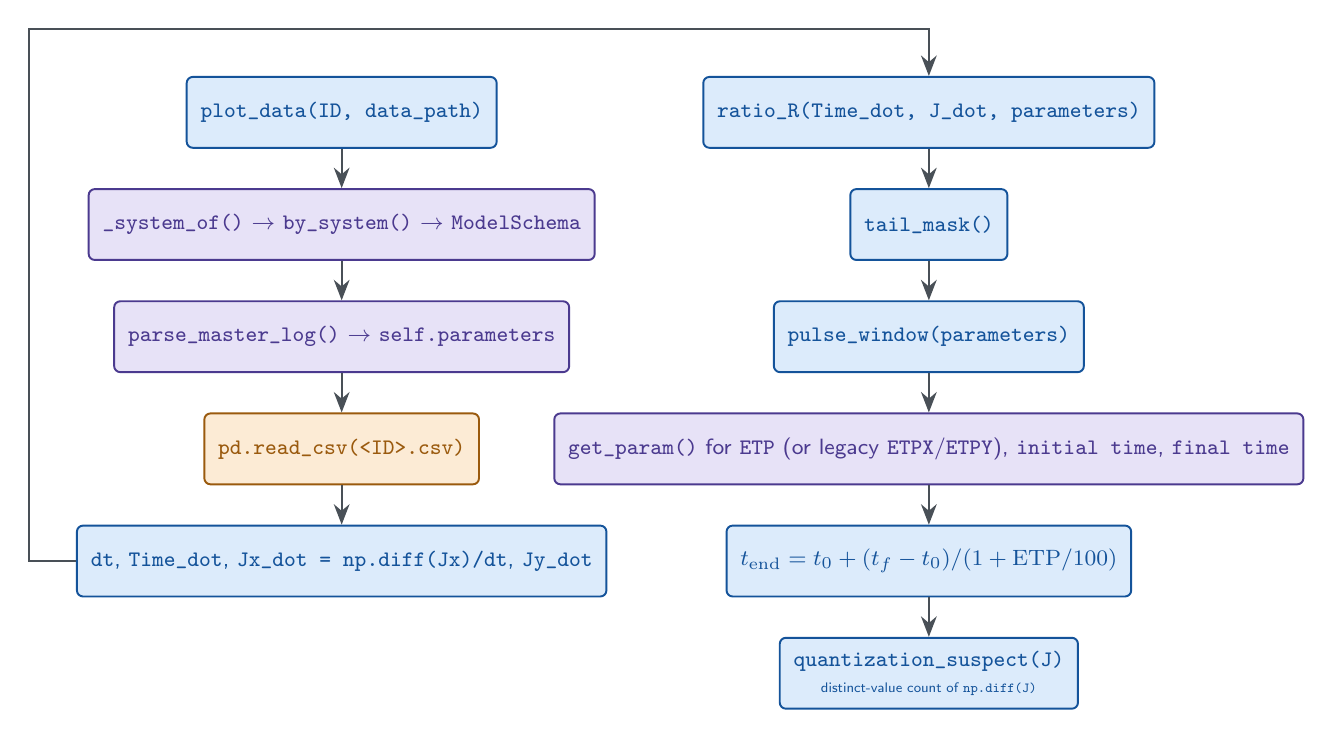
\begin{tikzpicture}[node distance=5mm and 11mm,
                    every node/.append style={font=\scriptsize\sffamily}]
  \node[py] (pd) {\fn{plot\uu data(ID, data\uu path)}};
  \node[idl, below=of pd] (ps) {\fn{\uu system\uu of()} $\rightarrow$ \fn{by\uu system()} $\rightarrow$ \fn{ModelSchema}};
  \node[idl, below=of ps] (pm) {\fn{parse\uu master\uu log()} $\rightarrow$ \fn{self.parameters}};
  \node[io,  below=of pm] (rd) {\fn{pd.read\uu csv(<ID>.csv)}};
  \node[py,  below=of rd] (dv) {\fn{dt}, \fn{Time\uu dot}, \fn{Jx\uu dot = np.diff(Jx)/dt}, \fn{Jy\uu dot}};

  \node[py, right=26mm of pd] (rr) {\fn{ratio\uu R(Time\uu dot, J\uu dot, parameters)}};
  \node[py, below=of rr] (tm) {\fn{tail\uu mask()}};
  \node[py, below=of tm] (pw) {\fn{pulse\uu window(parameters)}};
  \node[idl, below=of pw] (gp) {\fn{get\uu param()} for \fn{ETP} (or legacy \fn{ETPX}/\fn{ETPY}), \fn{initial time}, \fn{final time}};
  \node[py, below=of gp] (te) {$t_{\mathrm{end}} = t_0 + (t_f-t_0)/(1+\mathrm{ETP}/100)$};
  \node[py, below=of te] (qs) {\fn{quantization\uu suspect(J)}\\\tiny distinct-value count of \fn{np.diff(J)}};

  \foreach \a/\b in {pd/ps,ps/pm,pm/rd,rd/dv,rr/tm,tm/pw,pw/gp,gp/te,te/qs}
      \draw[flow] (\a) -- (\b);
  % routed around the outside; a direct link would cut through the get_param box
  \draw[flow] (dv.west) -- ++(-0.6,0) |- ([yshift=6mm]pd.north) -| (rr.north);
\end{tikzpicture}
\end{adjustbox}
\end{center}

\noindent
The post-pulse window is the only reason \fn{ETP} and \fn{final time} appear in
\code{parameters.txt} at all: the headline observable
$R=\max(\dot J)/\dot J(t_{\mathrm{end}})$ is measured on $(t_{\mathrm{end}},
t_f]$, and without those two fields it is not computable from the archive.

\clearpage

% ============================================================================
\section{Data flow and the memory boundary}\label{sec:mem}
% ============================================================================

\subsection{What the boundary actually is}

Figure~\ref{fig:mem} shows every place data changes representation. There are
three distinct memory regions and they are never mapped into one another.

\begin{figure}[H]
\centering
\begin{adjustbox}{width=\linewidth, max totalheight=0.72\textheight, center}
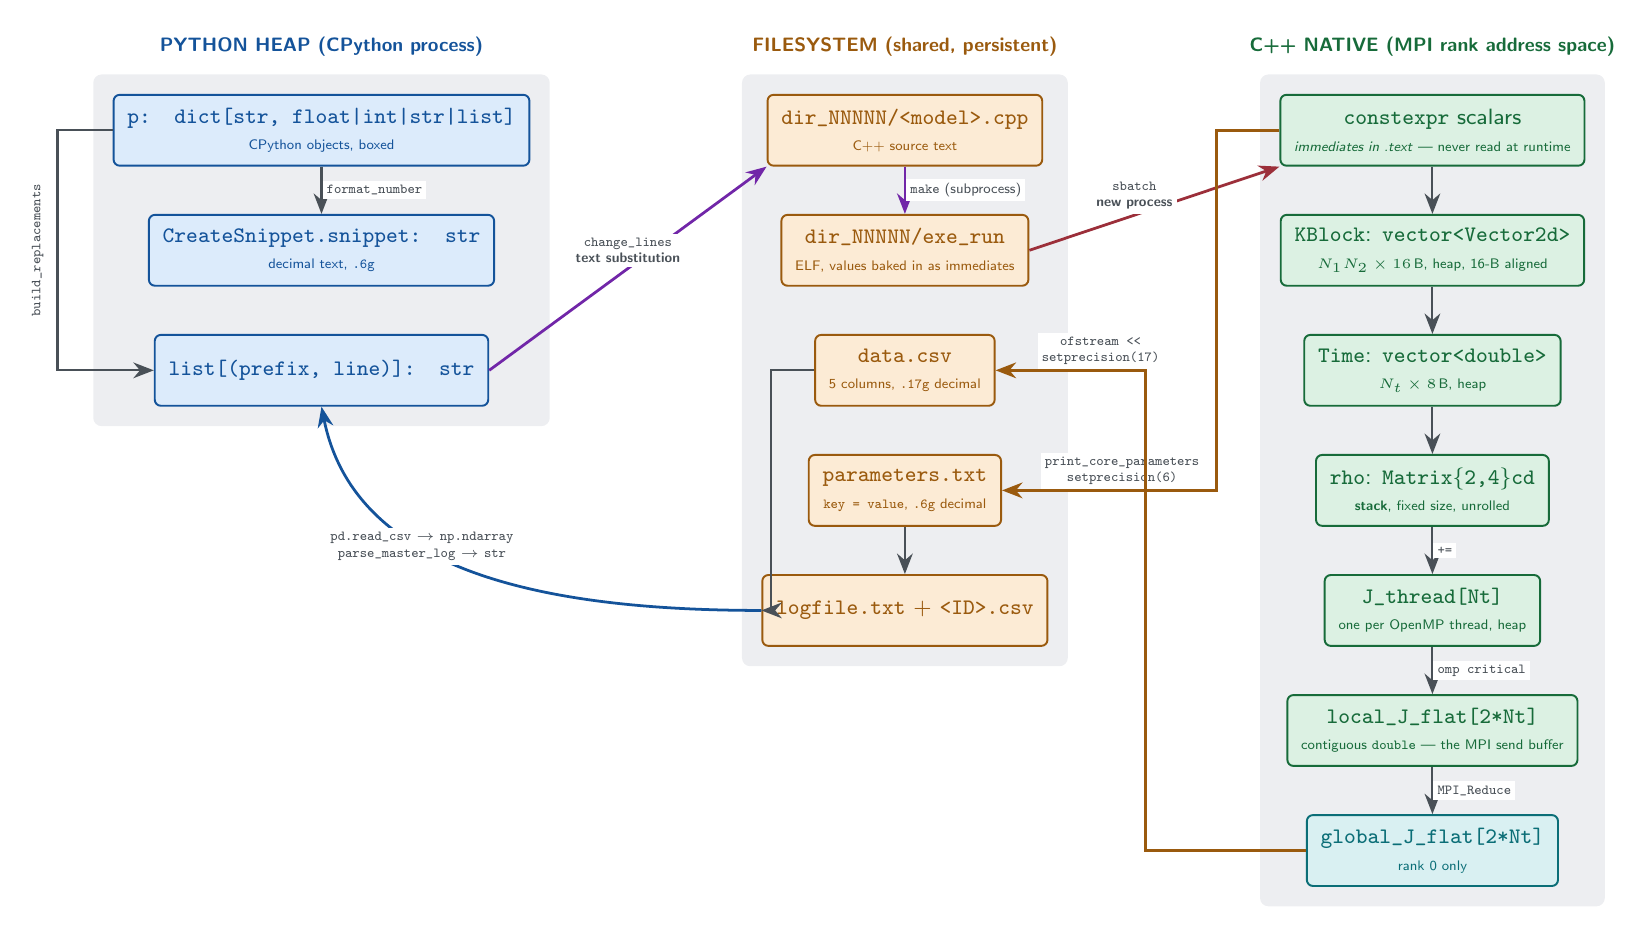
\begin{tikzpicture}[node distance=6mm and 10mm,
                    every node/.append style={font=\scriptsize\sffamily}]

% ---------------- region 1 : Python heap ------------------------------------
\node[py] (dict) {\fn{p: dict[str, float|int|str|list]}\\\tiny CPython objects, boxed};
\node[py, below=of dict] (snpt) {\fn{CreateSnippet.snippet: str}\\\tiny decimal text, \code{.6g}};
\node[py, below=of snpt] (rep) {\fn{list[(prefix, line)]: str}};

% ---------------- region 2 : filesystem -------------------------------------
\node[io, right=30mm of dict] (src) {\code{dir\uu NNNNN/<model>.cpp}\\\tiny C++ source text};
\node[io, below=of src] (exe) {\code{dir\uu NNNNN/exe\uu run}\\\tiny ELF, values baked in as immediates};
\node[io, below=of exe] (csv) {\code{data.csv}\\\tiny 5 columns, \code{.17g} decimal};
\node[io, below=of csv] (ptxt) {\code{parameters.txt}\\\tiny \code{key = value}, \code{.6g} decimal};
\node[io, below=of ptxt] (log) {\code{logfile.txt} + \code{<ID>.csv}};

% ---------------- region 3 : C++ native -------------------------------------
\node[cpp, right=30mm of src] (cst) {\fn{constexpr} scalars\\\tiny \emph{immediates in .text} --- never read at runtime};
\node[cpp, below=of cst] (kb) {\fn{KBlock}: \fn{vector<Vector2d>}\\\tiny $N_1N_2 \times 16$\,B, heap, 16-B aligned};
\node[cpp, below=of kb] (tv) {\fn{Time}: \fn{vector<double>}\\\tiny $N_t \times 8$\,B, heap};
\node[cpp, below=of tv] (rho) {\fn{rho}: \fn{Matrix\{2,4\}cd}\\\tiny \textbf{stack}, fixed size, unrolled};
\node[cpp, below=of rho] (jt) {\fn{J\uu thread[Nt]}\\\tiny one per OpenMP thread, heap};
\node[cpp, below=of jt] (flat) {\fn{local\uu J\uu flat[2*Nt]}\\\tiny contiguous \fn{double} --- the MPI send buffer};
\node[kern, below=of flat] (gl) {\fn{global\uu J\uu flat[2*Nt]}\\\tiny rank 0 only};

% ---------------- transitions -----------------------------------------------
\draw[flow] (dict) -- node[elab,right]{\fn{format\uu number}} (snpt);
% dict -> rep runs down a rail on the left so it does not cross the snippet box
\node[coordinate] (pyrail) at ([xshift=-7mm]dict.west) {};
\draw[flow] (dict.west) -- (pyrail) |- (rep.west);
\node[elab, rotate=90, anchor=south] at ([xshift=-1.2mm]pyrail |- snpt) {\fn{build\uu replacements}};
\draw[flow, draw=BindInk, line width=1.0pt] (rep.east) --
      node[elab,above,align=center]{\fn{change\uu lines}\\\tiny\textbf{text substitution}} (src.south west);
\draw[flow, draw=BindInk, line width=1.0pt] (src) --
      node[elab,right,align=center]{\fn{make} \tiny(subprocess)} (exe);
\draw[flow, draw=SchedInk, line width=1.0pt] (exe.east) --
      node[elab,pos=0.42,above,align=center]{\code{sbatch}\\\tiny\textbf{new process}} (cst.south west);
\draw[flow] (cst) -- (kb);
\draw[flow] (kb) -- (tv);
\draw[flow] (tv) -- (rho);
\draw[flow] (rho) -- node[elab,right]{\fn{+=}} (jt);
\draw[flow] (jt) -- node[elab,right]{\code{omp critical}} (flat);
\draw[flow] (flat) -- node[elab,right]{\fn{MPI\uu Reduce}} (gl);
% Both serialisation arrows run down their own rail in the inter-region gap,
% so neither cuts across a box.
\node[coordinate] (railA) at ([xshift=-8mm]cst.west) {};
\node[coordinate] (railB) at ([xshift=-17mm]cst.west) {};
\draw[flow, draw=IOInk, line width=1.0pt] (cst.west) -- (railA) |-
      node[elab,pos=0.72,above,align=center]{\fn{print\uu core\uu parameters}\\\tiny \fn{setprecision(6)}} (ptxt.east);
\draw[flow, draw=IOInk, line width=1.0pt] (gl.west) -- (gl.west -| railB) --
      (csv.east -| railB) --
      node[elab,pos=0.30,above,align=center]{\fn{ofstream <<}\\\tiny \fn{setprecision(17)}} (csv.east);
% csv -> log routed around parameters.txt rather than straight through it
\draw[flow] (csv.west) -- ++(-0.55,0) |- (log.west);
\draw[flow] (ptxt) -- (log);
\draw[flow, draw=PyInk, line width=1.0pt] (log.west) .. controls +(-3.0,0) and +(0.4,-2.0) ..
      node[elab,pos=0.6,align=center]{\fn{pd.read\uu csv} $\rightarrow$ \fn{np.ndarray}\\\fn{parse\uu master\uu log} $\rightarrow$ \fn{str}} (rep.south);

% ---------------- region frames ---------------------------------------------
\begin{scope}[on background layer]
  \node[band, fit=(dict)(snpt)(rep), inner sep=7pt] (r1) {};
  \node[band, fit=(src)(exe)(csv)(ptxt)(log), inner sep=7pt] (r2) {};
  \node[band, fit=(cst)(kb)(tv)(rho)(jt)(flat)(gl), inner sep=7pt] (r3) {};
\end{scope}
\node[above=1mm of r1, font=\scriptsize\bfseries\sffamily, text=PyInk]  {PYTHON HEAP (CPython process)};
\node[above=1mm of r2, font=\scriptsize\bfseries\sffamily, text=IOInk]  {FILESYSTEM (shared, persistent)};
\node[above=1mm of r3, font=\scriptsize\bfseries\sffamily, text=CppInk] {C++ NATIVE (MPI rank address space)};

\end{tikzpicture}
\end{adjustbox}
\caption{Data-flow and memory-boundary diagram. The three regions are separated
by process boundaries. Purple arrows are build-time transitions (text
substitution, compilation), the red arrow is a process launch, orange arrows
are serialisation, and the blue arrow is deserialisation. \textbf{No arrow on
this diagram is a pointer hand-off}; every crossing is mediated by decimal
text on disk.}
\label{fig:mem}
\end{figure}


\subsection{The precision contract}\label{sec:precision}

Because every crossing is decimal text, numerical identity across the boundary
is a formatting agreement. Two different agreements are in force, for two
different reasons.

\begin{center}
\scriptsize
\begin{tabular}{@{}L{0.15\textwidth} L{0.22\textwidth} L{0.21\textwidth} L{0.34\textwidth}@{}}
\toprule
\textbf{Payload} & \textbf{C++ writes} & \textbf{Python reads} & \textbf{Why} \\
\midrule
\code{parameters.txt}\newline (user parameters)
 & \fn{std::\brk setprecision(6)}
 & \fn{format\uu number} $=$ \fn{format(x,\brk ".6g")}
 & Matching is \emph{exact string equality} --- both sides of every comparison go
   through \fn{format\uu number}, so there is no float tolerance anywhere.
   Neither number may change alone. \\
\addlinespace
\code{data.csv}\newline (results)
 & \fn{std::\brk setprecision(17)},\newline deliberately \emph{not} \fn{std::\brk fixed}
 & \fn{pd.read\uu csv} $\rightarrow$ \fn{float64}
 & Full round-trip precision. General format is required because $J_y$ spans
   $\sim10^{-18}$ to $10^{-7}$; fixed notation would flush the small end to
   zero. \\
\bottomrule
\end{tabular}
\end{center}

\begin{keybox}[title={Historical consequence, recorded here because it is invisible in the code}]
Runs archived before 2026-08 were written at the stream default of 6
significant figures. Where $J$ is large and slowly varying, consecutive samples
became identical after rounding, so \fn{np.diff(J)/dt} measured the rounding
step rather than a derivative. This affects $J_x$ in 29 of the 38 archived
four-band runs; $J_y$ is unaffected everywhere and all 61 two-band runs are
clean. \fn{observables.quantization\uu suspect()} flags the condition by the
distinct-value count of \fn{np.diff(J)}.
\end{keybox}

\subsection{Native memory inside one rank}

\begin{figure}[H]
\centering
\begin{adjustbox}{width=\linewidth, max totalheight=0.80\textheight, center}
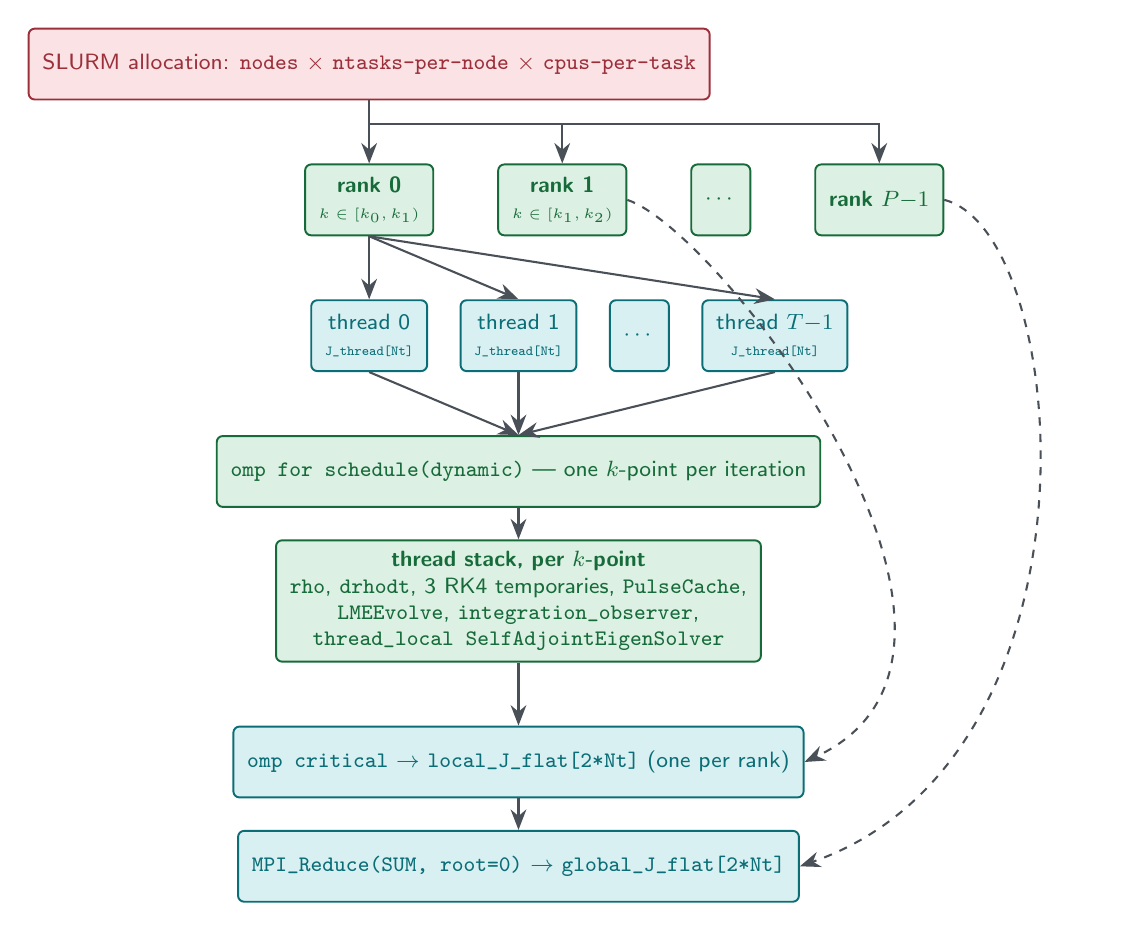
\begin{tikzpicture}[node distance=4mm and 8mm,
                    every node/.append style={font=\scriptsize\sffamily}]

  \node[sched] (slurm) {SLURM allocation: \fn{nodes} $\times$ \fn{ntasks-per-node} $\times$ \fn{cpus-per-task}};

  \node[cpp, below=8mm of slurm] (r0) {\textbf{rank 0}\\\tiny $k \in [k_0,k_1)$};
  \node[cpp, right=of r0] (r1) {\textbf{rank 1}\\\tiny $k \in [k_1,k_2)$};
  \node[cpp, right=of r1] (rd) {$\cdots$};
  \node[cpp, right=of rd] (rn) {\textbf{rank $P{-}1$}};

  \node[kern, below=8mm of r0] (t0) {thread 0\\\tiny \fn{J\uu thread[Nt]}};
  \node[kern, right=4mm of t0] (t1) {thread 1\\\tiny \fn{J\uu thread[Nt]}};
  \node[kern, right=4mm of t1] (t2) {$\cdots$};
  \node[kern, right=4mm of t2] (t3) {thread $T{-}1$\\\tiny \fn{J\uu thread[Nt]}};

  \node[cpp, below=8mm of t1] (kloop) {\code{omp for schedule(dynamic)} --- one $k$-point per iteration};
  \node[cpp, below=of kloop] (stack) {\textbf{thread stack, per $k$-point}\\
        \fn{rho}, \fn{drhodt}, 3 RK4 temporaries, \fn{PulseCache},\\
        \fn{LMEEvolve}, \fn{integration\uu observer},\\
        \fn{thread\uu local SelfAdjointEigenSolver}};

  \node[kern, below=8mm of stack] (crit) {\code{omp critical} $\rightarrow$ \fn{local\uu J\uu flat[2*Nt]} (one per rank)};
  \node[kern, below=of crit] (mred) {\fn{MPI\uu Reduce(SUM, root=0)} $\rightarrow$ \fn{global\uu J\uu flat[2*Nt]}};

  \draw[flow] (slurm.south) -- ++(0,-0.3) -| (r0.north);
  \draw[flow] (slurm.south) -- ++(0,-0.3) -| (r1.north);
  \draw[flow] (slurm.south) -- ++(0,-0.3) -| (rn.north);
  \foreach \t in {t0,t1,t3} \draw[flow] (r0.south) -- (\t.north);
  \foreach \t in {t0,t1,t3} \draw[flow] (\t.south) -- (kloop.north);
  \draw[flow] (kloop) -- (stack);
  \draw[flow] (stack) -- (crit);
  \draw[flow] (crit) -- (mred);
  % the other ranks, abbreviated: same structure, folded into the same reduction
  \draw[flow, dashed] (r1.east) .. controls +(1.2,-0.4) and +(3.0,1.4) .. (crit.east);
  \draw[flow, dashed] (rn.east) .. controls +(1.6,-0.4) and +(4.0,1.4) .. (mred.east);
\end{tikzpicture}
\end{adjustbox}
\caption{Memory ownership inside one MPI rank. Everything above
\code{omp critical} is thread-private; the reduction is the only shared write.}
\end{figure}

\begin{keybox}[title={Reproducibility consequence}]
The \code{\#pragma omp critical} reduction sums thread contributions in
\emph{arrival order}, which is not deterministic. Repeated identical runs
therefore differ at $\sim10^{-14}$ relative. Compare results numerically, never
by checksum --- unless the comparison is deliberately pinned to a single rank
and a single thread, in which case arrival order is forced and output is
bit-reproducible.
\end{keybox}

\subsection{Buffer inventory}

\begin{center}
\scriptsize
\begin{tabular}{@{}L{0.23\textwidth} L{0.24\textwidth} L{0.17\textwidth} L{0.28\textwidth}@{}}
\toprule
\textbf{Buffer} & \textbf{Type} & \textbf{Size} & \textbf{Lifetime / owner} \\
\midrule
\fn{KBlock}            & \fn{vector<Vector2d>} & $N_1N_2 \times 16$\,B & \fn{main}, read-only, shared by all threads \\
\fn{Time}              & \fn{vector<double>}   & $N_t \times 8$\,B     & \fn{main}, copied into \fn{necessary\uu functions} \\
\fn{Ls}                & \fn{vector<Matrix\{2,4\}cd>} & $|L_s| \times 64$ or $256$\,B & namespace scope, read-only \\
\fn{rho}, RK4 temporaries & \fn{Matrix\{2,4\}cd}  & $4 \times 64$ or $256$\,B & thread stack, one $k$-point \\
\fn{J\uu thread}       & \fn{vector<Vector2d>} & $N_t \times 16$\,B    & one per OpenMP thread \\
\fn{local\uu J\uu flat}& \fn{vector<double>}   & $2N_t \times 8$\,B    & one per rank; the MPI send buffer \\
\fn{global\uu J\uu flat}& \fn{vector<double>}  & $2N_t \times 8$\,B    & rank 0 only \\
\fn{TotalChargeCurrent}& \fn{vector<Vector2d>} & $N_t \times 16$\,B    & rank 0 only; the source of \code{data.csv} \\
\bottomrule
\end{tabular}
\end{center}

\noindent The flattening of \fn{J\uu thread} (a vector of \fn{Vector2d}) into
\fn{local\uu J\uu flat} (a plain \fn{double} array) exists solely to give MPI a
contiguous, type-describable buffer: \fn{MPI\uu Reduce} is handed
\fn{MPI\uu DOUBLE} and a count of $2N_t$. It is the one place in the code where
a data structure is reshaped purely for a boundary's benefit.

\clearpage

% ============================================================================
\section{Invariants that hold the layers together}
% ============================================================================

Each item below is load-bearing: changing one alone breaks something elsewhere.

\begin{center}
\scriptsize
\begin{tabular}{@{}L{0.26\textwidth} L{0.68\textwidth}@{}}
\toprule
\textbf{Invariant} & \textbf{What depends on it} \\
\midrule
6 significant figures & C++ \fn{setprecision(6)} and Python \fn{".6g"} are two halves of one contract. Matching is exact string equality with no tolerance. \\
\addlinespace
Results at \fn{setprecision(17)}, not \fn{std::fixed} & $J_y$ spans $10^{-18}$ to $10^{-7}$; fixed notation would flush the small end to zero. \\
\addlinespace
Three field categories & \emph{Identifying} (in the file, in the match); \emph{present but ignored} (in the file, in \fn{DEFAULT\uu IGNORE\uu PATTERNS}); \emph{omitted} (absent, because the run gives them no meaning --- when \fn{A0Y == 0} there is no \fn{nuY}, and writing a stale one would make two physically identical runs stop matching). \\
\addlinespace
Matching is subset, never substring & \fn{query\uu lines.issubset(entry\uu lines)}. The entry may carry extra lines, which is what keeps pre-2026-08 runs (with \fn{ETPX}/\fn{ETPY}, without \fn{TIME\uu DIVISION}) reachable from a query built today. \\
\addlinespace
One \fn{ETP}, not \fn{ETPX}/\fn{ETPY} & Extra-time-percentage is a simulation knob, not a per-channel property; two of them made the post-pulse window ambiguous. \\
\addlinespace
Naming & Pulse axes are the suffixes \fn{X}/\fn{Y}, never \fn{\uu x}. Reciprocal vectors are \fn{b1}/\fn{b2}/\fn{k\uu origin}, never limits. Grid is \fn{N1}/\fn{N2}, never \fn{Nx}/\fn{Ny}. Units are natural ($\hbar = e = a = 1$) and never labelled. \\
\addlinespace
The \fn{System} string & A run-integrity fingerprint: line 1 of \code{parameters.txt}, asserted in C++ \fn{main}, checked by \fn{parse\uu master\uu log}. \\
\addlinespace
Run IDs & Random 5-digit numbers, no zero padding. \\
\addlinespace
\fn{change\uu lines} must never be lenient & It raises on an unmatched prefix. A silent miss means a job runs with the wrong parameter and lands in the archive labelled as something it is not. \\
\bottomrule
\end{tabular}
\end{center}

\subsection{The acceptance test}

Before any change to the identification layer:

\begin{center}\ttfamily\scriptsize
python3 analysis/tests/test\uu archive\uu roundtrip.py \hfill \# expect 99/99\\[2pt]
python3 -c "import sys; sys.path.insert(0,'analysis'); import models; \textbackslash\\
\hspace*{2em}print([models.verify\uu cpp\uu mirror(m) for m in models.MODELS])" \hfill \# expect [[], []]
\end{center}

\noindent The second reads \fn{print\uu core\uu parameters()} out of the
\code{.cpp} and asserts it still agrees with \code{analysis/models.py}.

% ============================================================================
\section{Build and run reference}
% ============================================================================

\subsection{Build}

\begin{center}\ttfamily\scriptsize
\begin{tabular}{@{}l l@{}}
make -C physics check                & verify toolchain and header paths for the detected host \\
make -C physics                      & build both models for the auto-detected host \\
make -C physics HOST=param two\uu band & force a host, build one model \\
make -C physics clean                & remove \code{build/} \\
\end{tabular}
\end{center}

\noindent \fn{HOST} is one of \fn{local}, \fn{param}, \fn{hpc}, auto-detected
from \fn{\$HOME}. Objects live in \code{build/\$(HOST)/} so a
\fn{-march=native} local build can never be linked into a cluster binary by
accident.

\subsection{Submit}

\begin{center}\ttfamily\scriptsize
\begin{tabular}{@{}l l@{}}
python3 workflow/generator\uu four\uu band.py --dry-run & prepare run dirs, stop before \fn{sbatch} \\
python3 workflow/generator\uu four\uu band.py           & full submission \\
python3 workflow/generator\uu two\uu band.py --host param & override host detection \\
\end{tabular}
\end{center}

\subsection{Data locations}

Outside the repository, never in git:

\begin{center}\ttfamily\scriptsize
\begin{tabular}{@{}l l@{}}
\textasciitilde/ComputationData/PostDoc/programming/new/data/ & \\
\quad two\uu band\uu model/\ \ <ID>.csv + logfile.txt  & 61 runs \\
\quad four\uu band\uu model/\ \ <ID>.csv + logfile.txt & 38 runs \\
\quad images/ & \\
\textasciitilde/temp\uu files\uu data/ & staging \\
\textasciitilde/research\uu backup/PostDoc/programming/new/data/ & mirror \\
\end{tabular}
\end{center}

\subsection{Repository tree}

\begin{center}\ttfamily\scriptsize
\begin{tabular}{@{}l@{}}
new/\\
\quad CLAUDE.md\ \ context.md\ \ README.md\ \ .gitignore\\
\quad physics/\\
\qquad Makefile\\
\qquad include/necessary\uu functions.h\\
\qquad src/necessary\uu functions.cpp\\
\qquad models/two\uu band.cpp\ \ models/four\uu band.cpp\\
\qquad build/\$(HOST)/\ \ \ \ \rmfamily(git-ignored)\ttfamily\\
\quad workflow/\\
\qquad hpc\uu config.py\ \ submit\uu utils.py\ \ Makefile.job\\
\qquad generator\uu two\uu band.py\ \ generator\uu four\uu band.py\\
\quad analysis/\\
\qquad models.py\ \ snippets.py\ \ data\uu utils.py\\
\qquad loaders.py\ \ observables.py\ \ plotstyle.py\\
\qquad tests/test\uu archive\uu roundtrip.py\\
\qquad notebooks/\ \ \ \ \rmfamily(git-ignored)\ttfamily\\
\quad docs/\ \ \ hpc\uu notes.md\ \ parameters.txt.sample\ \ code\uu architecture.tex\\
\quad mathematica/test.nb\\
\quad legacy/\ \ \ \rmfamily frozen; never built, never imported\ttfamily\\
\end{tabular}
\end{center}

\vfill
\begin{center}\footnotesize\sffamily\color{Slate}
End of blueprint.
\end{center}

\end{document}
